% foster_to_cauer_it.tex
% Dalla rete termica di Foster alla rete di Cauer: la trasformazione foster_to_cauer().
% Versione italiana di foster_to_cauer.tex (stessa struttura, stesse etichette, stesse equazioni e stesso codice).
% Template pwr-control (AAA_template_latex_settings); numeri e figure degli esempi svolti:
% foster_cauer_calc.py (con il modulo foster_cauer.py), che scrive foster_cauer_values.tex e figures/fig_*_it.pdf
% Compilazione: pdflatex foster_to_cauer_it.tex  (due volte, per i riferimenti)
% Rev. 00 - novembre 2026 - prima emissione
\documentclass[10pt,a4paper]{scrartcl}
\PassOptionsToPackage{main=italian}{babel}   % settings.tex carica babel con [british]: l'italiano diventa la lingua principale
\input{../../../../AAA_template_latex_settings/settings}
% il documento sta quattro livelli sotto la radice del repository: percorso del logo di settings.tex corretto qui
\rhead{\includegraphics[height=0.75cm]{../../../../AAA_template_latex_settings/pwr-control_logo_doc.png}}
\rfoot{\small Rev.~00}
\geometry{left=2.0cm, right=2.0cm}
\usepackage[european resistors, american inductors]{circuitikz}
\usepackage{listings}
\usepackage{icomma}   % virgola decimale nelle formule: 1,806 senza lo spazio della punteggiatura
\babelhyphenation[italian]{case data-sheet}   % prestiti inglesi: "case" non si divide, "datasheet" solo come data-sheet

\sisetup{output-decimal-marker={,},per-mode=symbol,range-phrase={\text{--}},range-units=single}
\setlist{nosep}
\setlength{\parindent}{0pt}
\setlength{\parskip}{3pt}
\allowdisplaybreaks
\captionsetup{font=small,labelfont=bf}
\renewcommand{\topfraction}{0.9}
\renewcommand{\bottomfraction}{0.9}
\renewcommand{\textfraction}{0.05}
\renewcommand{\floatpagefraction}{0.8}
\lstset{language=Python, basicstyle=\ttfamily\footnotesize, columns=fullflexible, keepspaces=true,
  numbers=left, numberstyle=\tiny\color{gray}, numbersep=6pt, xleftmargin=1.5em, frame=lines,
  framerule=0.4pt, rulecolor=\color{gray}, commentstyle=\color{gray!70!black}\itshape,
  keywordstyle=\color{blue!55!black}\bfseries, stringstyle=\color{orange!60!black}, showstringspaces=false}

% --- numeri degli esempi svolti (generati da foster_cauer_calc.py) ---
% Lo stesso file della versione inglese, letto sostituendo il punto decimale con la virgola: ogni macro \fc...
% si espande in un numero come 4,533, valido sia nel testo sia dentro \SI{}{} di siunitx.
\ExplSyntaxOn
\cs_new_protected:Npn \fcitdefine #1#2
  {
    \tl_set:Nn \l_tmpa_tl {#2}
    \tl_replace_all:Nnn \l_tmpa_tl { . } { , }
    \cs_gset_eq:NN #1 \l_tmpa_tl
  }
\ExplSyntaxOff
\begingroup
\let\newcommand\fcitdefine
% generated by foster_cauer_calc.py: do not edit by hand
\newcommand{\fcddRA}{4.533}
\newcommand{\fcddTA}{0.4406}
\newcommand{\fcddRcA}{0.980}
\newcommand{\fcddCcA}{3.53}
\newcommand{\fcddCfA}{97.2}
\newcommand{\fcddRCcA}{3.46}
\newcommand{\fcddRB}{2.255}
\newcommand{\fcddTB}{0.1045}
\newcommand{\fcddRcB}{1.058}
\newcommand{\fcddCcB}{8.43}
\newcommand{\fcddCfB}{46.3}
\newcommand{\fcddRCcB}{8.92}
\newcommand{\fcddRC}{0.868}
\newcommand{\fcddTC}{0.0092}
\newcommand{\fcddRcC}{3.757}
\newcommand{\fcddCcC}{25.2}
\newcommand{\fcddCfC}{10.6}
\newcommand{\fcddRCcC}{94.71}
\newcommand{\fcddRD}{0.345}
\newcommand{\fcddTD}{0.0022}
\newcommand{\fcddRcD}{2.206}
\newcommand{\fcddCcD}{144.4}
\newcommand{\fcddCfD}{6.38}
\newcommand{\fcddRCcD}{318.68}
\newcommand{\fcddRth}{8.001}
\newcommand{\fcddDelay}{0.56}
\newcommand{\fcddStored}{557}
\newcommand{\fcddThetaA}{8.001}
\newcommand{\fcddThetaB}{7.021}
\newcommand{\fcddThetaC}{5.964}
\newcommand{\fcddThetaD}{2.206}
\newcommand{\fcddCcSum}{181.6}
\newcommand{\fcddCfSum}{160.5}
\newcommand{\fcddCfSeries}{3.53}
\newcommand{\fcddMone}{2.2416}
\newcommand{\fcddErrPoly}{4\times 10^{-16}}
\newcommand{\fcddErrBid}{1\times 10^{-15}}
\newcommand{\fcddErrRt}{3\times 10^{-15}}
\newcommand{\fcddErrZ}{2\times 10^{-15}}
\newcommand{\fcddRpar}{8.03}
\newcommand{\fcddKa}{1.806}
\newcommand{\fcddRsSuma}{14.45}
\newcommand{\fcddRsaA}{1.769}
\newcommand{\fcddRsaB}{1.909}
\newcommand{\fcddRsaC}{6.784}
\newcommand{\fcddRsaD}{3.984}
\newcommand{\fcddCsaB}{4.67}
\newcommand{\fcddCsaC}{14.0}
\newcommand{\fcddCsaD}{80.0}
\newcommand{\fcddKb}{2.241}
\newcommand{\fcddRsSumb}{17.93}
\newcommand{\fcddRsbA}{2.196}
\newcommand{\fcddRsbB}{2.370}
\newcommand{\fcddRsbC}{8.422}
\newcommand{\fcddRsbD}{4.945}
\newcommand{\fcddCsbB}{3.76}
\newcommand{\fcddCsbC}{11.2}
\newcommand{\fcddCsbD}{64.4}
\newcommand{\fcddShareA}{55.4}
\newcommand{\fcdtRA}{3.587}
\newcommand{\fcdtTA}{0.4299}
\newcommand{\fcdtRcA}{0.354}
\newcommand{\fcdtCcA}{2.88}
\newcommand{\fcdtCfA}{119.8}
\newcommand{\fcdtRCcA}{1.02}
\newcommand{\fcdtRB}{0.838}
\newcommand{\fcdtTB}{0.0405}
\newcommand{\fcdtRcB}{0.421}
\newcommand{\fcdtCcB}{4.01}
\newcommand{\fcdtCfB}{48.3}
\newcommand{\fcdtRCcB}{1.69}
\newcommand{\fcdtRC}{0.505}
\newcommand{\fcdtTC}{0.0028}
\newcommand{\fcdtRcC}{1.449}
\newcommand{\fcdtCcC}{32.0}
\newcommand{\fcdtCfC}{5.54}
\newcommand{\fcdtRCcC}{46.41}
\newcommand{\fcdtRD}{0.069}
\newcommand{\fcdtTD}{0.0005}
\newcommand{\fcdtRcD}{2.775}
\newcommand{\fcdtCcD}{110.0}
\newcommand{\fcdtCfD}{7.25}
\newcommand{\fcdtRCcD}{305.37}
\newcommand{\fcdtRth}{4.999}
\newcommand{\fcdtDelay}{0.47}
\newcommand{\fcdtStored}{474}
\newcommand{\fcdtThetaA}{4.999}
\newcommand{\fcdtThetaB}{4.645}
\newcommand{\fcdtThetaC}{4.224}
\newcommand{\fcdtThetaD}{2.775}
\newcommand{\fcdtCcSum}{149.0}
\newcommand{\fcdtCfSum}{181.0}
\newcommand{\fcdtCfSeries}{2.88}
\newcommand{\fcdtMone}{1.5774}
\newcommand{\fcdtErrPoly}{2\times 10^{-16}}
\newcommand{\fcdtErrBid}{9\times 10^{-16}}
\newcommand{\fcdtErrRt}{6\times 10^{-15}}
\newcommand{\fcdtErrZ}{5\times 10^{-15}}
\newcommand{\fcdtRpar}{5.00}
\newcommand{\fcdtKa}{2.000}
\newcommand{\fcdtRsSuma}{10.00}
\newcommand{\fcdtRsaA}{0.708}
\newcommand{\fcdtRsaB}{0.843}
\newcommand{\fcdtRsaC}{2.897}
\newcommand{\fcdtRsaD}{5.550}
\newcommand{\fcdtCsaB}{2.00}
\newcommand{\fcdtCsaC}{16.0}
\newcommand{\fcdtCsaD}{55.0}
\newcommand{\fcdtKb}{2.000}
\newcommand{\fcdtRsSumb}{10.00}
\newcommand{\fcdtRsbA}{0.708}
\newcommand{\fcdtRsbB}{0.843}
\newcommand{\fcdtRsbC}{2.897}
\newcommand{\fcdtRsbD}{5.550}
\newcommand{\fcdtCsbB}{2.00}
\newcommand{\fcdtCsbC}{16.0}
\newcommand{\fcdtCsbD}{55.0}
\newcommand{\fcdtShareA}{50.0}
\newcommand{\fccpP}{15}
\newcommand{\fccpT}{0.5}
\newcommand{\fccpE}{7.5}
\newcommand{\fccpTjI}{98}
\newcommand{\fccpTjC}{101}
\newcommand{\fccpTjF}{141}
\newcommand{\fccpDiff}{41}
\newcommand{\fccpTcC}{14}
\newcommand{\fccpTcF}{44}
\newcommand{\fccpTcFzero}{38}
\newcommand{\fccpQten}{199}
\newcommand{\fccpQend}{33}
\newcommand{\fccpEstored}{6.40}
\newcommand{\fccpEstoredPct}{85}
\newcommand{\fccpRch}{5}
\newcommand{\fccpCbar}{620}
\newcommand{\fcsySaDevF}{20}
\newcommand{\fcsySaAbsF}{20}
\newcommand{\fcsySaDevT}{1.6}
\newcommand{\fcsySaDevX}{-46}
\newcommand{\fcsySaAbsX}{46}
\newcommand{\fcsyScDevF}{19}
\newcommand{\fcsyScAbsF}{19}
\newcommand{\fcsyScDevT}{1.6}
\newcommand{\fcsyScDevX}{-55}
\newcommand{\fcsyScAbsX}{55}
\newcommand{\fcsyNodes}{109}
\newcommand{\fcsyRth}{7.62}
\newcommand{\fcsyRa}{14.2}
\newcommand{\fcsyRc}{17.0}
\newcommand{\fcsyCsi}{2.56}
\newcommand{\fcsyCmo}{28.0}
\newcommand{\fcsyCcu}{171}
\newcommand{\fcsyCtot}{202}
\newcommand{\fcsyModes}{109}
\newcommand{\fcsyCninetyNine}{194}
\newcommand{\fcsyCmax}{2\times 10^{10}}
\newcommand{\fcsyCoFull}{2.56}
\newcommand{\fcsyErrFull}{5\times 10^{-13}}
\newcommand{\fcsyFitThreeErr}{2.36}
\newcommand{\fcsyFitThreeCo}{3.06}
\newcommand{\fcsyFitThreeCsum}{70}
\newcommand{\fcsyFitThreeTmin}{2.40}
\newcommand{\fcsyFitThreeDev}{12.6}
\newcommand{\fcsyFitFourErr}{0.28}
\newcommand{\fcsyFitFourCo}{2.84}
\newcommand{\fcsyFitFourCsum}{106}
\newcommand{\fcsyFitFourTmin}{1.32}
\newcommand{\fcsyFitFourDev}{6.8}
\newcommand{\fcsyFitFiveErr}{0.05}
\newcommand{\fcsyFitFiveCo}{2.78}
\newcommand{\fcsyFitFiveCsum}{115}
\newcommand{\fcsyFitFiveTmin}{0.90}
\newcommand{\fcsyFitFiveDev}{6.0}
\newcommand{\fcsyFitSixErr}{0.01}
\newcommand{\fcsyFitSixCo}{2.75}
\newcommand{\fcsyFitSixCsum}{133}
\newcommand{\fcsyFitSixTmin}{0.66}
\newcommand{\fcsyFitSixDev}{4.7}
\newcommand{\fcsyFRA}{4.764}
\newcommand{\fcsyFTA}{0.3310}
\newcommand{\fcsyRcFA}{0.761}
\newcommand{\fcsyCcFA}{2.84}
\newcommand{\fcsyFRB}{1.900}
\newcommand{\fcsyFTB}{0.0545}
\newcommand{\fcsyRcFB}{1.059}
\newcommand{\fcsyCcFB}{5.80}
\newcommand{\fcsyFRC}{0.708}
\newcommand{\fcsyFTC}{0.0063}
\newcommand{\fcsyRcFC}{2.882}
\newcommand{\fcsyCcFC}{16.7}
\newcommand{\fcsyFRD}{0.251}
\newcommand{\fcsyFTD}{0.0013}
\newcommand{\fcsyRcFD}{2.920}
\newcommand{\fcsyCcFD}{80.5}
\newcommand{\fcsyKa}{1.833}
\newcommand{\fcsyKc}{2.200}
\newcommand{\fcsyHalfZm}{6.76}
\newcommand{\fcsyHalfZc}{7.11}
\newcommand{\fcsyHalfZx}{6.57}
\newcommand{\fcsyHalfZf}{9.48}
\newcommand{\fcsyHalfZi}{6.57}
\newcommand{\fcsyHalfEc}{5.2}
\newcommand{\fcsyHalfEx}{-2.8}
\newcommand{\fcsyHalfEf}{40}
\newcommand{\fcsyHalfEi}{-2.8}
\newcommand{\fcsyMaxEc}{6.8}
\newcommand{\fcsyMinEc}{-0.28}
\newcommand{\fcsyMaxEx}{90}
\newcommand{\fcsyMaxEf}{871}
\newcommand{\fcsyTmaxEf}{1}
\newcommand{\fcsyShortA}{-6}
\newcommand{\fcsyShortB}{-9}
\newcommand{\fcssSaDevF}{20}
\newcommand{\fcssSaAbsF}{20}
\newcommand{\fcssSaDevT}{1.6}
\newcommand{\fcssSaDevX}{-3}
\newcommand{\fcssSaAbsX}{3}
\newcommand{\fcssScDevF}{20}
\newcommand{\fcssScAbsF}{20}
\newcommand{\fcssScDevT}{1.6}
\newcommand{\fcssScDevX}{-3}
\newcommand{\fcssScAbsX}{3}
\newcommand{\fcssNodes}{114}
\newcommand{\fcssRth}{6.98}
\newcommand{\fcssRa}{14.2}
\newcommand{\fcssRc}{14.2}
\newcommand{\fcssCsi}{2.56}
\newcommand{\fcssCmo}{32.0}
\newcommand{\fcssCcu}{171}
\newcommand{\fcssCtot}{206}
\newcommand{\fcssModes}{57}
\newcommand{\fcssCninetyNine}{198}
\newcommand{\fcssCmax}{2\times 10^{1}}
\newcommand{\fcssCoFull}{2.56}
\newcommand{\fcssErrFull}{1\times 10^{-12}}
\newcommand{\fcssFitThreeErr}{3.35}
\newcommand{\fcssFitThreeCo}{3.71}
\newcommand{\fcssFitThreeCsum}{68}
\newcommand{\fcssFitThreeTmin}{1.58}
\newcommand{\fcssFitThreeDev}{14.7}
\newcommand{\fcssFitFourErr}{0.44}
\newcommand{\fcssFitFourCo}{3.21}
\newcommand{\fcssFitFourCsum}{109}
\newcommand{\fcssFitFourTmin}{0.81}
\newcommand{\fcssFitFourDev}{7.4}
\newcommand{\fcssFitFiveErr}{0.05}
\newcommand{\fcssFitFiveCo}{2.98}
\newcommand{\fcssFitFiveCsum}{119}
\newcommand{\fcssFitFiveTmin}{0.52}
\newcommand{\fcssFitFiveDev}{6.2}
\newcommand{\fcssFitSixErr}{0.01}
\newcommand{\fcssFitSixCo}{2.91}
\newcommand{\fcssFitSixCsum}{132}
\newcommand{\fcssFitSixTmin}{0.44}
\newcommand{\fcssFitSixDev}{5.1}
\newcommand{\fcssFRA}{4.870}
\newcommand{\fcssFTA}{0.3488}
\newcommand{\fcssRcFA}{0.376}
\newcommand{\fcssCcFA}{3.21}
\newcommand{\fcssFRB}{1.525}
\newcommand{\fcssFTB}{0.0580}
\newcommand{\fcssRcFB}{0.838}
\newcommand{\fcssCcFB}{7.47}
\newcommand{\fcssFRC}{0.422}
\newcommand{\fcssFTC}{0.0057}
\newcommand{\fcssRcFC}{2.817}
\newcommand{\fcssCcFC}{18.6}
\newcommand{\fcssFRD}{0.159}
\newcommand{\fcssFTD}{0.0008}
\newcommand{\fcssRcFD}{2.945}
\newcommand{\fcssCcFD}{79.6}
\newcommand{\fcssKa}{2.000}
\newcommand{\fcssKc}{2.000}
\newcommand{\fcssHalfZm}{5.98}
\newcommand{\fcssHalfZc}{6.31}
\newcommand{\fcssHalfZx}{5.96}
\newcommand{\fcssHalfZf}{8.72}
\newcommand{\fcssHalfZi}{5.82}
\newcommand{\fcssHalfEc}{5.5}
\newcommand{\fcssHalfEx}{-0.3}
\newcommand{\fcssHalfEf}{46}
\newcommand{\fcssHalfEi}{-2.7}
\newcommand{\fcssMaxEc}{7.4}
\newcommand{\fcssMinEc}{-0.44}
\newcommand{\fcssMaxEx}{1.1}
\newcommand{\fcssMaxEf}{1125}
\newcommand{\fcssTmaxEf}{1}
\newcommand{\fcssShortA}{-12}
\newcommand{\fcssShortB}{-19}
\newcommand{\fcacBadOne}{26}
\newcommand{\fcacPctOne}{24}
\newcommand{\fcacSixOne}{18}
\newcommand{\fcacBidOne}{1\times 10^{-14}}
\newcommand{\fcacBadTwo}{40}
\newcommand{\fcacPctTwo}{36}
\newcommand{\fcacSixTwo}{28}
\newcommand{\fcacBidTwo}{8\times 10^{-15}}
\newcommand{\fcacBadFour}{--}
\newcommand{\fcacPctFour}{--}
\newcommand{\fcacSixFour}{48}
\newcommand{\fcacBidFour}{8\times 10^{-15}}
\newcommand{\fcacBadEight}{--}
\newcommand{\fcacPctEight}{--}
\newcommand{\fcacSixEight}{--}
\newcommand{\fcacBidEight}{7\times 10^{-15}}
\newcommand{\fcacBidMax}{1\times 10^{-14}}
\newcommand{\fcmpDigits}{200}

\endgroup

% --- abbreviazioni ---
\newcommand{\Zth}{Z_\mathrm{th}}
\newcommand{\Zjc}{Z_\mathrm{th(j-c)}}
\newcommand{\Rth}{R_\mathrm{th}}
\newcommand{\Rjc}{R_\mathrm{th(j-c)}}
\newcommand{\Rch}{R_\mathrm{th(c-h)}}
\newcommand{\Tj}{T_\mathrm{j}}
\newcommand{\Tc}{T_\mathrm{c}}
\newcommand{\Rpar}{R_\mathrm{par}}
\newcommand{\diff}{\mathrm{d}}
\newcommand{\lc}{\operatorname{lc}}
\newcommand{\KkW}{\si{\kelvin\per\kilo\watt}}
\newcommand{\JK}{\si{\joule\per\kelvin}}
\newcommand{\ms}{\si{\milli\second}}
\newcommand{\code}[1]{\texttt{#1}}

% =============================================================
%  DATI DEL DOCUMENTO (frontespizio: AAA_template_latex_settings/titlepage.tex)
% =============================================================
\newcommand{\DocCategory}{Nota tecnica}
\newcommand{\DocField}{Elettronica di potenza e sistemi di controllo}
\newcommand{\DocTitle}{%
	{\fontsize{20}{24}\selectfont\bfseries Dalla rete termica di Foster} \\[16pt]
	{\fontsize{16}{20}\selectfont\bfseries alla rete di Cauer di un dispositivo di potenza}
}
\newcommand{\DocSubtitle}{La trasformazione \texttt{foster\_to\_cauer()}: sviluppo in frazione continua dell'impedenza termica transitoria del datasheet, una rete a scala per lato di un press-pack raffreddato su due lati, accuratezza numerica e limiti}
\newcommand{\DocAuthor}{Davide Bagnara}
\newcommand{\DocRevision}{00}
\newcommand{\DocDate}{Novembre 2026}
\newcommand{\DocAbstract}{%
I datasheet danno l'impedenza termica transitoria giunzione--case di un dispositivo di potenza come rete di Foster, una somma di termini esponenziali misurata con il case mantenuto a temperatura costante. La rete di Foster riproduce esattamente quella misura e nient'altro: i suoi nodi non sono punti del dispositivo, e tutto il calore ne esce dal case nell'istante stesso in cui è generato. Appena il case è collegato a qualcosa che si scalda, un contatto e una barra o un dissipatore, la rete di Foster vi invia il calore troppo presto e sovrastima la temperatura di giunzione. La rete di Cauer, una rete a scala di resistenze e capacità termiche dalla giunzione al case, ha la stessa impedenza con il case a temperatura costante, ma il suo calore raggiunge il case con il ritardo dovuto al calore accumulato lungo il percorso, e il suo nodo di case può essere collegato a qualsiasi rete esterna. La nota descrive la trasformazione dall'una all'altra così come la esegue la funzione \texttt{foster\_to\_cauer()}: la somma di Foster scritta come rapporto di due polinomi, lo sviluppo in frazione continua del suo inverso, ogni passo con la sua riga di codice, perché tutti gli elementi risultano positivi, la forma chiusa della prima sezione, le grandezze che ogni conversione corretta conserva e con cui la si può verificare. Tratta l'accuratezza numerica dello sviluppo polinomiale, che è al livello dell'errore di arrotondamento per i pochi termini di un datasheet e fallisce per molte costanti di tempo ravvicinate, e un'alternativa stabile per bidiagonalizzazione; la suddivisione dell'impedenza con raffreddamento su due lati in una rete a scala per lato, con le resistenze su singolo lato del datasheet; e ciò che la rete a scala non contiene, verificato su un press-pack di cui si conoscono gli strati. Esempi svolti: un diodo raddrizzatore da \SI{2}{\kilo\volt} e un tiristore da \SI{1.8}{\kilo\volt} in press-pack, con il diodo serrato tra due barre di rame. Gli script Python di supporto riproducono ogni numero e ogni figura.
}
\newcommand{\RevisionHistory}{%
	00 & Novembre 2026 & Prima emissione (versione italiana della Rev.~00 in inglese). & \DocAuthor \\
}
\newcommand{\MetaLabelA}{Repository}
\newcommand{\MetaValueAUrl}{https://github.com/pwr-control/repositories-documentation.git}
\newcommand{\MetaValueALabel}{repositories-documentation.git}
\newcommand{\MetaLabelB}{Calcolo}
\newcommand{\MetaValueB}{Python 3 / NumPy, SciPy (\texttt{foster\_cauer\_calc.py})}

\begin{document}
\input{../../../../AAA_template_latex_settings/titlepage}
\tableofcontents
\newpage

%=====================================================================
\section{Scopo e risultati}
\label{sec:scope}
Il datasheet di un dispositivo di potenza dà l'impedenza termica transitoria dalla giunzione al case, $\Zjc(t)$: la sovratemperatura della giunzione per un gradino di perdite di un watt, con il case mantenuto a temperatura costante. La dà come curva e come tabella di $n$ coppie $R_i$, $\tau_i$ della forma analitica
\begin{equation}
\Zjc(t) = \sum_{i=1}^{n} R_i \left(1 - e^{-t/\tau_i}\right) ,
\label{eq:zth}
\end{equation}
che è la risposta al gradino di una rete di Foster: $n$ celle, ciascuna una resistenza $R_i$ in parallelo a una capacità $C_i = \tau_i/R_i$, in serie dalla giunzione al case (Fig.~\ref{fig:networks}a).

La rete di Foster è esatta per la prova da cui proviene e solo per quella. I suoi nodi interni non sono punti del dispositivo, e ogni cella è percorsa dall'intera potenza: il calore esce dalla rete al case nell'istante in cui è generato. In un convertitore il case non è mantenuto a temperatura costante: poggia su un contatto e su un dissipatore o una barra, che si scaldano. Una rete di Foster collegata a essi vi immette il calore troppo presto e la giunzione risulta troppo calda. La rete di Cauer, una rete a scala di capacità termiche verso massa e di resistenze in serie (Fig.~\ref{fig:networks}b), ha la stessa impedenza quando il case è a temperatura costante, ed è il modello a parametri concentrati di un percorso termico monodimensionale: il calore raggiunge il case con il ritardo di ciò che si accumula lungo il percorso, e al nodo di case si può collegare qualsiasi cosa.

La funzione \code{foster\_to\_cauer()} trasforma la tabella di Foster di un datasheet nella rete a scala di Cauer. È stata scritta per la verifica termica di uno stack crowbar di dispositivi press-pack serrati tra barre di rame, dove il case è la faccia di un polo appoggiata su una barra di capacità termica finita. Questa nota descrive che cosa fa e perché funziona (Sez.~\ref{sec:networks} e~\ref{sec:transform}), quanto è accurata e come fare meglio quando non lo è (Sez.~\ref{sec:numerics}), come un dispositivo raffreddato su due lati si suddivide in una rete a scala per lato (Sez.~\ref{sec:sides}), e che cosa la rete a scala contiene e non contiene (Sez.~\ref{sec:examples} e~\ref{sec:synthetic}). La Sez.~\ref{sec:procedure} riassume la procedura.

\subsection*{I risultati in breve}
\begin{enumerate}
\item La somma di Foster è un rapporto di polinomi, $Z(s) = N(s)/D(s)$ con $D = \prod_i (1+s\tau_i)$. La rete a scala di Cauer è lo sviluppo in frazione continua di $Y = 1/Z = D/N$ attorno a $s = \infty$: si estrae il polo all'infinito dell'ammettenza, una capacità; si inverte; si estrae il valore all'infinito dell'impedenza, una resistenza; si inverte; si ripete $n$ volte (Sez.~\ref{sec:cf}). Ogni elemento è un rapporto di coefficienti direttivi. La funzione fa esattamente questo con i polinomi di \code{numpy} (Sez.~\ref{sec:code}).
\item Tutti gli elementi sono positivi, e la rete a scala è unica, perché $Z(s)$ è l'impedenza di una rete RC: poli reali negativi con residui positivi (Sez.~\ref{sec:positive}). La prima sezione ha una forma chiusa: $C_1 = 1/\sum_i (R_i/\tau_i)$, inverso della pendenza iniziale di $\Zjc$, e $R_1 = \bigl(\sum_i R_i/\tau_i\bigr)^2 \big/ \sum_i R_i/\tau_i^2$.
\item Una conversione corretta conserva $\sum R_k = \sum R_i = \Rjc$, dà $C_1 = 1/\sum (R_i/\tau_i)$, conserva il momento del primo ordine $\sum_k C_k \theta_k^2 = \sum_i R_i\tau_i$ ($\theta_k$ resistenza dal nodo $k$ al case) e restituisce le $R_i$, $\tau_i$ dagli autovalori della rete a scala (Sez.~\ref{sec:checks}). Sono le verifiche da eseguire su ogni rete convertita.
\item Per i quattro termini di un datasheet lo sviluppo polinomiale è esatto a meno dell'arrotondamento ($\fcddErrPoly$ per il diodo degli esempi). Perde cifre quando le costanti di tempo sono molte e ravvicinate: con le costanti di tempo distribuite su una decade gli elementi sono errati di oltre \SI{1}{\percent} da $n = \fcacPctOne$ termini e negativi da $n = \fcacBadOne$; su due decadi da $n = \fcacPctTwo$ e da $n = \fcacBadTwo$ (Fig.~\ref{fig:accuracy}). Una bidiagonalizzazione della forma agli autovalori dà la stessa rete a scala con soli prodotti e quozienti, al livello dell'arrotondamento per qualsiasi numero di termini (Sez.~\ref{sec:bidiag}).
\item Un press-pack raffreddato su due lati ha una sola $\Zjc$ per i due lati e una $\Rth$ per lato. Ogni lato diventa la stessa rete a scala con ogni $R$ moltiplicata e ogni $C$ divisa per $k = R_\mathrm{lato}/\Rpar$; la capacità di giunzione $C_1$ è in comune. Poiché $\sum 1/k = 1$, le due reti a scala in parallelo restituiscono esattamente l'impedenza con raffreddamento su due lati (Sez.~\ref{sec:sides}).
\item Per il diodo degli esempi tra due barre di rame, un impulso di \SI{\fccpP}{\kilo\watt} per \SI{\fccpT}{\second} innalza la giunzione di \SI{\fccpTjC}{\kelvin} con le reti a scala di Cauer e di \SI{\fccpTjF}{\kelvin} con la rete di Foster sulle barre: \SI{\fccpDiff}{\kelvin} di troppo. Con la rete a scala, alla fine dell'impulso nelle barre entra solo il \SI{\fccpQend}{\percent} della potenza; in media il calore lascia il dispositivo \SI{\fcddDelay}{\second} dopo essere stato generato (Sez.~\ref{sec:onbars}).
\item Verificata su un press-pack di strati noti, una rete a scala ricavata da un fit a quattro termini come quello di un datasheet dà la temperatura di giunzione sulle barre entro \SI{\fcsyMinEc}{\percent} e $+\fcsyMaxEc$~\% rispetto al modello (per eccesso, a meno dell'accuratezza del fit per impulsi brevi), la rete di Foster $+\fcsyHalfEf$~\% per un impulso di \SI{0.5}{\second} e molto di più per impulsi più brevi. Alla rete a scala di un fit da datasheet manca parte della capacità termica vicina al case, che la prova con il case a temperatura costante quasi non vede; l'errore è a favore di sicurezza. La stessa capacità mancante rende le curve su singolo lato delle reti a scala suddivise fino al \SI{\fcsySaDevF}{\percent} troppo alte (Sez.~\ref{sec:synthetic}).
\item Più termini non sono sempre meglio: quando i due lati del dispositivo differiscono, la rete a scala esatta della curva con raffreddamento su due lati termina con sezioni di capacità fino a $\fcsyCmax$~\JK{} che non corrispondono ad alcun materiale. Sulle barre agiscono come un secondo dissipatore e la giunzione risulta fino al \SI{\fcsyMaxEx}{\percent} troppo fredda. Una rete a scala ricavata da un fit di pochi termini non ha sezioni di questo tipo (Sez.~\ref{sec:missing}).
\end{enumerate}

%=====================================================================
\section{Nomenclatura}
\label{sec:nomenclature}
\begin{center}\small
\begin{tabular}{@{}>{$}l<{$}>{\raggedright\arraybackslash}p{6.4cm}>{$}l<{$}>{\raggedright\arraybackslash}p{6.1cm}@{}}
\toprule
\Zjc(t) & impedenza termica transitoria giunzione--case, risposta al gradino di \SI{1}{\watt} & R_i,\ \tau_i & resistenza e costante di tempo dell'$i$-esimo termine di Foster \\
Z(s),\ Y(s) & impedenza e ammettenza termica nel dominio di Laplace, $Y = 1/Z$ & C_i^\mathrm{F} & capacità di una cella di Foster, $\tau_i/R_i$ \\
\Rjc & resistenza termica giunzione--case, $Z(0) = \sum R_i$ & R_k,\ C_k & resistenza e capacità termica della $k$-esima sezione della rete a scala di Cauer \\
\Rch & resistenza di contatto case--dissipatore (o barra) & \theta_k & resistenza dal nodo $k$ della rete a scala al case, $\sum_{j\ge k} R_j$ \\
\Tj,\ \Tc & temperatura virtuale di giunzione, temperatura del case & n & numero di termini (di sezioni) \\
p(t) & potenza dissipata nel dispositivo & D(s),\ N(s) & denominatore e numeratore di $Z(s)$ \\
\lambda_i,\ w_i & poli e residui di $Z$: $1/\tau_i$ e $R_i/\tau_i$ & \lc(\cdot) & coefficiente direttivo di un polinomio \\
\Rpar & parallelo delle resistenze su singolo lato & k & fattore di scala di un lato, $R_\mathrm{lato}/\Rpar$ \\
G,\ \mathbf{C} & matrice delle conduttanze e matrice delle capacità di una rete & M & matrice simmetrica $\mathbf{C}^{-1/2} G\, \mathbf{C}^{-1/2}$ \\
\bottomrule
\end{tabular}
\end{center}
Le grandezze termiche seguono l'analogia elettrica: la temperatura è una tensione, il flusso di calore una corrente, la massa del circuito equivalente è la temperatura di riferimento. Tutte le temperature sono sovratemperature rispetto alla temperatura iniziale, che è anche quella di un dissipatore ideale. Le resistenze sono date in \KkW{} come nei datasheet, le capacità in \JK.

%=====================================================================
\section{Le due reti}
\label{sec:networks}

\subsection{Che cosa misura il datasheet}
L'impedenza termica transitoria si misura con un gradino di potenza nel dispositivo e il case mantenuto a temperatura costante, di solito su un dissipatore raffreddato ad acqua; la temperatura di giunzione è quella virtuale, ricavata da un parametro elettrico sensibile alla temperatura. La curva copre una finestra temporale di qualche decade, tipicamente da \SI{1}{\milli\second} a \SI{10}{\second} o più, e la tabella \eqref{eq:zth} ne è un fit con pochi termini esponenziali. Per un press-pack il datasheet dà la curva e la tabella per il raffreddamento su due lati, e la resistenza a regime anche per il raffreddamento dal solo lato anodo e dal solo lato catodo.

Ne seguono due fatti che contano per il resto della nota. La tabella è un fit: altri insiemi di $R_i$, $\tau_i$, con più o meno termini, approssimano la stessa curva entro la sua accuratezza, e fuori dalla finestra della misura la tabella è un'estrapolazione. E la tabella descrive una sola condizione al contorno, il case a temperatura costante; ogni altra condizione al contorno è al di fuori di ciò che è stato misurato.

\subsection{Rete di Foster}
Nel dominio di Laplace la tabella \eqref{eq:zth} è
\begin{equation}
Z(s) = \sum_{i=1}^{n} \frac{R_i}{1 + s\tau_i} = \sum_{i=1}^{n} \frac{w_i}{s + \lambda_i} , \qquad \lambda_i = \frac{1}{\tau_i} , \quad w_i = \frac{R_i}{\tau_i} ,
\label{eq:zfoster}
\end{equation}
la somma delle impedenze di $n$ celle parallelo $R_i \parallel C_i^\mathrm{F}$, con $C_i^\mathrm{F} = \tau_i/R_i$, in serie (Fig.~\ref{fig:networks}a). Tre proprietà di questa rete decidono come la si può usare.
\begin{itemize}
\item Le celle sono in serie, quindi ciascuna è percorsa dall'intera potenza $p(t)$: il flusso di calore che dall'ultima cella entra nel case è $p(t)$ in ogni istante. Per quanto il case può vedere, lungo il percorso non si accumula nulla.
\item La temperatura di un nodo interno è la somma delle cadute delle celle che lo precedono. Non è la temperatura di alcuno strato del dispositivo, e le capacità $C_i^\mathrm{F}$ non sono capacità termiche di nulla: stanno in parallelo alle resistenze, non tra un nodo e la massa.
\item La temperatura di giunzione è $\Tj(t) = \Tc(t) + \int_0^t \Zjc'(t-u)\,p(u)\,\diff u$ qualunque cosa accada al case. Con il case a temperatura costante è corretto. Con il case su un dissipatore che si scalda, il dissipatore è forzato da $p(t)$ stessa invece che dal calore che lo raggiunge davvero, che arriva più tardi e smussato.
\end{itemize}
Il terzo punto è la consueta somma di un'impedenza giunzione--case e di una case--ambiente, ciascuna forzata dall'intera potenza. Negli esempi di questa nota tale somma dà un limite superiore valido, ed è d'uso comune per questo motivo, ma può essere lontana dalla temperatura reale (Sez.~\ref{sec:onbars} e~\ref{sec:synthetic}).

\begin{figure}[htb]
\centering
\begin{circuitikz}[scale=0.82, transform shape, european resistors]
\begin{scope}
\node[anchor=west] at (-0.6,2.2) {\textbf{(a)} Rete di Foster};
\draw (0,-1.6) node[ground]{} to[I, l=$p(t)$, invert] (0,0);
\draw (0,0) node[circ]{} node[above left]{$\Tj$} -- (0.5,0);
\foreach \i/\x in {1/0.5,2/2.7,3/4.9,4/7.1} {
  \draw (\x,0) -- (\x,0.6) to[R, l=$R_\i$] (\x+1.7,0.6) -- (\x+1.7,0);
  \draw (\x,0) -- (\x,-0.6) to[C, l_=$C^\mathrm{F}_\i$] (\x+1.7,-0.6) -- (\x+1.7,0);
}
\draw (2.2,0) -- (2.7,0); \draw (4.4,0) -- (4.9,0); \draw (6.6,0) -- (7.1,0);
\draw (8.8,0) -- (9.6,0) node[circ]{} node[above]{$\Tc$} -- (10.2,0) to[V, l=$\Tc$ imposta, invert] (10.2,-1.6) node[ground]{};
\end{scope}
\begin{scope}[yshift=-5.0cm]
\node[anchor=west] at (-0.6,2.0) {\textbf{(b)} Rete di Cauer};
\draw (0,-1.6) node[ground]{} to[I, l=$p(t)$, invert] (0,0);
\draw (0,0) node[circ]{} node[above left]{$\Tj$} -- (1.6,0) node[circ]{};
\draw (1.6,0) to[C, l_=$C_1$] (1.6,-1.6) node[ground]{};
\draw (1.6,0) to[R, l=$R_1$] (3.6,0) node[circ]{};
\draw (3.6,0) to[C, l_=$C_2$] (3.6,-1.6) node[ground]{};
\draw (3.6,0) to[R, l=$R_2$] (5.6,0) node[circ]{};
\draw (5.6,0) to[C, l_=$C_3$] (5.6,-1.6) node[ground]{};
\draw (5.6,0) to[R, l=$R_3$] (7.6,0) node[circ]{};
\draw (7.6,0) to[C, l_=$C_4$] (7.6,-1.6) node[ground]{};
\draw (7.6,0) to[R, l=$R_4$] (9.6,0) node[circ]{} node[below left]{$\Tc$} -- (10.2,0) to[V, l=$\Tc$ imposta, invert] (10.2,-1.6) node[ground]{};
\draw[densely dashed, gray] (9.6,0) -- (9.6,0.9) node[above, black, font=\small]{o qualsiasi rete esterna};
\end{scope}
\end{circuitikz}
\caption{Le due reti di una $\Zjc$ a quattro termini. (a) Foster: celle in serie, ciascuna percorsa dall'intera potenza; solo il nodo di giunzione ha un significato fisico. (b) Cauer: capacità termiche verso massa e resistenze in serie, un percorso termico monodimensionale a parametri concentrati dalla giunzione al case. Con il case a temperatura costante le due reti hanno la stessa impedenza; solo la rete a scala può essere collegata a una rete esterna al case.}
\label{fig:networks}
\end{figure}

\subsection{Rete di Cauer}
La rete di Cauer (Fig.~\ref{fig:networks}b) è una rete a scala: il nodo 1, la giunzione, con la capacità $C_1$ verso massa, la resistenza $R_1$ verso il nodo 2 con $C_2$, e così via fino a $R_n$, che termina al case. È il modello a parametri concentrati di un percorso termico a strati piani: $C_k$ è la capacità termica di una fetta del percorso, $R_k$ la resistenza tra due fette. La sua impedenza, con il case a temperatura costante, è la frazione continua
\begin{equation}
Z(s) = \cfrac{1}{sC_1 + \cfrac{1}{R_1 + \cfrac{1}{sC_2 + \cfrac{1}{R_2 + \cdots + \cfrac{1}{sC_n + \cfrac{1}{R_n}}}}}} .
\label{eq:zcauer}
\end{equation}
Data $Z(s)$ della forma \eqref{eq:zfoster}, la rete a scala con la stessa impedenza esiste, ha elementi positivi ed è unica (Sez.~\ref{sec:positive}). Con il case a temperatura costante le due reti non si possono distinguere dalla giunzione: stessa $\Zjc(t)$, stessa temperatura di giunzione per qualsiasi forma d'onda di potenza. Differiscono all'interno, e la differenza si vede appena il case non è più a temperatura costante.
\begin{itemize}
\item Nella rete a scala il calore raggiunge il case solo dopo aver scaldato le capacità lungo il percorso. Per un gradino di potenza il flusso di calore nel case parte da zero; il calore accumulato nel dispositivo a regime è $p\sum_k C_k\theta_k$, dove $\theta_k = \sum_{j\geq k} R_j$ è la resistenza dal nodo $k$ al case. La stessa somma è il ritardo medio con cui il calore lascia il case dopo essere stato generato.
\item Il nodo di case è un nodo come gli altri: vi si può collegare una resistenza di contatto, un dissipatore, una barra o un secondo dispositivo, e la rete dell'intero stack è ancora una rete di capacità verso massa e di resistenze, risolvibile con qualsiasi simulatore circuitale o termico.
\item La rete a scala non è il dispositivo. È il percorso monodimensionale a parametri concentrati che ha l'impedenza misurata; quanto le sue sezioni si avvicinino agli strati reali è l'argomento della Sez.~\ref{sec:synthetic}.
\end{itemize}

%=====================================================================
\section{La trasformazione}
\label{sec:transform}

\subsection{La somma di Foster come rapporto di polinomi}
Ridotta a denominatore comune, la \eqref{eq:zfoster} è
\begin{equation}
Z(s) = \frac{N(s)}{D(s)} , \qquad D(s) = \prod_{i=1}^{n} (1 + s\tau_i) , \qquad N(s) = \sum_{k=1}^{n} R_k \prod_{j \neq k} (1 + s\tau_j) .
\label{eq:nd}
\end{equation}
$D$ ha grado $n$, $N$ grado $n-1$. L'ammettenza $Y = D/N$ cresce quindi come $s$ ad alta frequenza: ha un polo all'infinito, che è la capacità $C_1$ del nodo di giunzione.

\subsection{Frazione continua}
\label{sec:cf}
Si scriva l'ammettenza al passo $k$ come $Y_k = D_k/N_k$ con $\deg D_k = \deg N_k + 1$; all'inizio $D_1 = D$ e $N_1 = N$. Un passo estrae una capacità e una resistenza:
\begin{align}
C_k &= \frac{\lc D_k}{\lc N_k} , & P_k &= D_k - s\,C_k\, N_k , & Y_k - sC_k &= \frac{P_k}{N_k} , \label{eq:stepC}\\
R_k &= \frac{\lc N_k}{\lc P_k} , & Q_k &= N_k - R_k\, P_k , & \frac{N_k}{P_k} - R_k &= \frac{Q_k}{P_k} , \label{eq:stepR}
\end{align}
e l'ammettenza successiva è $Y_{k+1} = P_k/Q_k$, cioè $D_{k+1} = P_k$, $N_{k+1} = Q_k$. Qui $\lc$ è il coefficiente direttivo, il coefficiente della potenza più alta di $s$.

I gradi spiegano ogni passo. $D_k$ e $sN_k$ hanno lo stesso grado, e $C_k$ è scelto in modo che i loro termini di grado massimo si elidano: $P_k$ ha il grado di $N_k$, e $P_k/N_k$ ha un valore finito all'infinito. Il suo inverso $N_k/P_k$ è un'impedenza con valore finito all'infinito, $R_k$; estrarla elide di nuovo il termine di grado massimo, e $Q_k$ ha un grado in meno di $P_k$, così che $P_k/Q_k$ ha di nuovo un polo all'infinito. Ogni passo abbassa di uno entrambi i gradi; dopo $n$ passi $N_n$ è una costante, $P_n$ è una costante e $Q_n = 0$. Nella rete a scala questo si legge
\begin{equation}
Y_k = sC_k + \cfrac{1}{R_k + \cfrac{1}{Y_{k+1}}} ,
\end{equation}
che, ripetuta, è la \eqref{eq:zcauer}: $C_k$ è la capacità dal nodo $k$ verso massa, $R_k$ la resistenza verso il nodo $k+1$, e $1/Y_{k+1}$ l'impedenza del resto della rete a scala vista dal nodo $k+1$.

\subsection{Perché gli elementi sono positivi}
\label{sec:positive}
La $Z(s)$ della \eqref{eq:zfoster} ha poli semplici sul semiasse reale negativo con residui positivi $w_i$, è nulla all'infinito e positiva in zero: è l'impedenza di ingresso di una rete RC a una porta. Queste funzioni hanno tre proprietà usate qui \cite{foster1924,cauer1926,guillemin1957}: zeri e poli sono reali, semplici e alternati sul semiasse reale negativo; l'inverso di un'impedenza RC è un'ammettenza RC, della forma $Y(s) = s\,c_\infty + g_0 + \sum_j g_j\, s/(s+\sigma_j)$ con coefficienti non negativi; e ciò che resta dopo aver estratto da una funzione RC un polo all'infinito, o il suo valore all'infinito, è ancora una funzione RC, con un polo in meno.

Dai primi termini dello sviluppo di $Z$ attorno all'infinito,
\begin{equation}
Z(s) = \frac{1}{s}\sum_i w_i - \frac{1}{s^2}\sum_i \frac{w_i}{\tau_i} + O\!\left(s^{-3}\right) , \qquad
Y(s) = \frac{s}{\sum_i w_i} + \frac{\sum_i w_i/\tau_i}{\bigl(\sum_i w_i\bigr)^2} + O\!\left(s^{-1}\right) ,
\end{equation}
la prima sezione si ottiene in forma chiusa,
\begin{equation}
C_1 = \frac{1}{\sum_i R_i/\tau_i} , \qquad R_1 = \frac{\bigl(\sum_i R_i/\tau_i\bigr)^2}{\sum_i R_i/\tau_i^2} ,
\label{eq:first}
\end{equation}
entrambe positive. $C_1$ è l'inverso della pendenza iniziale di $\Zjc(t)$: per $t$ molto più breve della più piccola $\tau_i$, $\Zjc(t) \approx t/C_1$, e tutte le reti con questa $Z(s)$ si comportano all'inizio come un'unica capacità $C_1$. È la capacità termica efficace della nota sull'active clamping di questo repository \cite{activeclamping}, e la serie delle capacità di Foster, $1/C_1 = \sum_i 1/C_i^\mathrm{F}$.

Quindi $Y - sC_1$ è un'ammettenza RC senza polo all'infinito e con valore positivo all'infinito, $1/R_1$; il suo inverso meno $R_1$ è un'impedenza RC nulla all'infinito, della stessa forma di $Z$ con $n-1$ poli; e il ragionamento si ripete. Tutte le $C_k$ e $R_k$ sono positive, ce ne sono esattamente $n$ di ciascun tipo, e poiché ogni passo è obbligato la rete a scala è unica. È la prima forma canonica di Cauer \cite{cauer1926}.

\subsection{La funzione, riga per riga}
\label{sec:code}
La funzione riceve la tabella di Foster e restituisce la rete a scala, $R$ nella stessa unità della tabella e $C$ in J/K quando $R$ è in K/W e $\tau$ in secondi. I polinomi sono array \code{numpy} di coefficienti per potenze decrescenti di $s$, quindi il coefficiente direttivo è l'elemento \code{[0]}.
\begin{lstlisting}
def foster_to_cauer(R, tau):
    n = len(R)
    D = np.array([1.0])
    for ti in tau:
        D = np.polymul(D, [ti, 1.0])                              # D = prod (tau_i s + 1)
    N = np.zeros(1)
    for k in range(n):
        term = np.array([R[k]])
        for j in range(n):
            if j != k:
                term = np.polymul(term, [tau[j], 1.0])
        N = np.polyadd(N, term)                                    # N = sum R_k prod_{j!=k} (tau_j s + 1)
    num, den = D, N                      # Y(s) = num / den, deg(num) = deg(den) + 1
    Cs, Rs = [], []
    for _ in range(n):
        C = num[0] / den[0]
        rem = np.polysub(num, np.polymul([C, 0.0], den))[1:]      # Y - s C   (leading term cancels)
        Rk = den[0] / rem[0]
        rem2 = np.polysub(den, Rk * rem)[1:]                       # Z - R     (leading term cancels)
        Cs.append(C); Rs.append(Rk)
        num, den = rem, rem2
    return np.array(Rs), np.array(Cs)
\end{lstlisting}
\begin{itemize}
\item Le righe 3--12 costruiscono $D$ e $N$ della \eqref{eq:nd}; \code{[ti, 1.0]} è il polinomio $\tau_i s + 1$.
\item Riga 13: \code{num}, \code{den} sono $D_k$, $N_k$ dell'ammettenza corrente.
\item La riga 16 è $C_k = \lc D_k/\lc N_k$ della \eqref{eq:stepC}; la riga 17 forma $P_k = D_k - sC_kN_k$ (\code{[C, 0.0]} è il polinomio $C_k s$) e ne scarta il primo coefficiente, che è nullo in aritmetica esatta ed è un residuo di arrotondamento in virgola mobile.
\item La riga 18 è $R_k = \lc N_k/\lc P_k$ della \eqref{eq:stepR}; la riga 19 forma $Q_k = N_k - R_kP_k$ e ne scarta il primo coefficiente per la stessa ragione.
\item La riga 21 passa alla sezione successiva, $D_{k+1} = P_k$, $N_{k+1} = Q_k$. All'ultimo passaggio \code{rem2} è vuoto: $Q_n = 0$.
\end{itemize}
Il primo coefficiente viene scartato, non verificato: per l'elisione la funzione si affida alla teoria, e in virgola mobile non controlla mai quanto fosse grande il residuo. È innocuo per i pochi termini di un datasheet ed è lì che si perde l'accuratezza quando i termini sono molti (Sez.~\ref{sec:numerics}). L'ordine dei termini in ingresso non conta, perché $D$ e $N$ sono simmetrici rispetto a essi.

\subsection{Dalla rete a scala alla tabella}
\label{sec:inverse}
La trasformazione inversa è una verifica e uno strumento: trasforma una rete a scala nella tabella di Foster che serve a un simulatore o a un confronto con il datasheet. Le equazioni ai nodi della rete a scala con il case a temperatura costante sono $\mathbf{C}\,\dot{\boldsymbol\theta} = -G\boldsymbol\theta + \mathbf{e}_1 p$, con $\mathbf{C} = \operatorname{diag}(C_k)$ e $G$ tridiagonale, $G_{kk} = 1/R_{k-1} + 1/R_k$ ($1/R_0 = 0$) e $G_{k,k+1} = G_{k+1,k} = -1/R_k$. Con la matrice simmetrica $M = \mathbf{C}^{-1/2}G\,\mathbf{C}^{-1/2} = Q\Lambda Q^\mathsf{T}$,
\begin{equation}
Z(s) = \mathbf{e}_1^\mathsf{T}(s\mathbf{C} + G)^{-1}\mathbf{e}_1 = \frac{1}{C_1}\sum_{i=1}^{n} \frac{q_{1i}^2}{s + \lambda_i}
\quad\Longrightarrow\quad
\tau_i = \frac{1}{\lambda_i} , \qquad R_i = \frac{q_{1i}^2}{C_1\lambda_i} ,
\label{eq:eig}
\end{equation}
dove $q_{1i}$ è la prima componente dell'$i$-esimo autovettore unitario. Le costanti di tempo di Foster sono date dagli autovalori della rete a scala, non dai prodotti $R_kC_k$ delle sue sezioni. Il confronto della \eqref{eq:eig} con la \eqref{eq:zfoster} ridà $C_1 = 1/\sum_i w_i$, poiché i $q_{1i}^2$ hanno somma uno.

\subsection{Che cosa conserva ogni conversione corretta}
\label{sec:checks}
Quattro grandezze dipendono dalla sola $Z(s)$ e si possono calcolare da entrambe le parti di una conversione:
\begin{enumerate}
\item la resistenza, $Z(0)$: $\sum_k R_k = \sum_i R_i = \Rjc$;
\item la capacità di giunzione \eqref{eq:first}: $C_1 = 1/\sum_i (R_i/\tau_i)$, pari anche a $1/\sum_i (1/C_i^\mathrm{F})$;
\item il momento del primo ordine, $-Z'(0)$, che è l'area compresa tra $\Rjc$ e la curva $\Zjc(t)$: dal lato di Foster $\sum_i R_i\tau_i$; dal lato della rete a scala $\boldsymbol\theta^\mathsf{T}\mathbf{C}\,\boldsymbol\theta = \sum_k C_k\theta_k^2$, con $\boldsymbol\theta = G^{-1}\mathbf{e}_1$ le temperature dei nodi a regime per un watt, $\theta_k = \sum_{j\ge k} R_j$;
\item i poli e i residui: gli autovalori e le prime componenti degli autovettori della rete a scala \eqref{eq:eig} restituiscono le $\tau_i$ e le $R_i$.
\end{enumerate}
La capacità totale non è tra queste: $\sum_k C_k$ e $\sum_i C^\mathrm{F}_i$ sono numeri diversi ($\fcddCcSum$ e $\fcddCfSum$~\JK{} per il diodo della Sez.~\ref{sec:examples}), e nessuno dei due è la capacità termica del dispositivo (Sez.~\ref{sec:missing}).

%=====================================================================
\section{Accuratezza numerica}
\label{sec:numerics}

\subsection{Dove lo sviluppo polinomiale perde cifre}
Ogni passo delle \eqref{eq:stepC}--\eqref{eq:stepR} sottrae due polinomi i cui termini di grado massimo sono uguali per costruzione, e l'informazione sta in ciò che resta. I coefficienti di $D$ e $N$ sono funzioni simmetriche elementari delle $\tau_i$; lavorare con essi significa lavorare con i momenti $\sum_i w_i/\tau_i^m$ dello spettro delle costanti di tempo, come mostra la \eqref{eq:first} per la prima sezione. Il passaggio dai momenti a una frazione continua è la via classica ai polinomi ortogonali, ed è mal condizionato: il suo numero di condizionamento cresce esponenzialmente con il numero di termini, tanto più rapidamente quanto più le costanti di tempo sono vicine tra loro \cite{gautschi2004}. Quando le costanti di tempo sono poche e distanti, come in un datasheet, ogni coefficiente è dominato da un diverso prodotto di costanti di tempo e le sottrazioni perdono poche cifre; quando sono molte e vicine, i resti diventano differenze di numeri quasi uguali e le cifre si esauriscono. Un secondo limite è il campo della doppia precisione: il coefficiente direttivo di $D$ è $\prod_i\tau_i$, che va in underflow con un centinaio di termini con costanti di tempo fino a $10^{-8}$~s.

\subsection{Un'alternativa stabile: la bidiagonalizzazione}
\label{sec:bidiag}
La forma agli autovalori \eqref{eq:eig} offre una via che non costruisce mai un polinomio. Per la rete a scala, $G = E\,\operatorname{diag}(1/R_k)\,E^\mathsf{T}$, con $E$ la matrice bidiagonale inferiore con $1$ sulla diagonale e $-1$ sotto di essa (la matrice di incidenza delle resistenze, l'ultima delle quali va al case). Quindi
\begin{equation}
M = BB^\mathsf{T} , \qquad B = \mathbf{C}^{-1/2} E\, \operatorname{diag}(R_k)^{-1/2} , \qquad B_{kk} = \frac{1}{\sqrt{C_kR_k}} , \quad B_{k+1,k} = -\frac{1}{\sqrt{C_{k+1}R_k}} ,
\end{equation}
e $B$ è il fattore bidiagonale inferiore di $M$, i cui valori singolari sono $\sqrt{\lambda_i}$. Dati i poli $\lambda_i$ e il vettore $\mathbf{u}$ delle prime componenti degli autovettori, $u_i = \sqrt{w_i C_1}$, la bidiagonalizzazione di Golub--Kahan di $A = \operatorname{diag}\bigl(\sqrt{\lambda_i}\bigr)$ avviata da $\mathbf{u}$ \cite{golubkahan1965,paige1982} restituisce la matrice bidiagonale con diagonale $\alpha_k$ e sottodiagonale $\beta_{k+1}$ tale che $BB^\mathsf{T}$ ha autovalori $\lambda_i$ e autovettori con prime componenti $u_i$. I segni degli elementi non influiscono sull'impedenza, e la rete a scala si ricava con soli prodotti e quozienti di numeri positivi:
\begin{equation}
C_1 = \frac{1}{\sum_i w_i} , \qquad R_k = \frac{1}{\alpha_k^2\, C_k} , \qquad C_{k+1} = \frac{1}{\beta_{k+1}^2\, R_k} .
\label{eq:bidiag}
\end{equation}
Con la riortogonalizzazione completa la bidiagonalizzazione lavora direttamente sullo spettro e non forma mai i momenti; nelle prove della Fig.~\ref{fig:accuracy} la sua rete a scala è al livello dell'arrotondamento per qualsiasi numero di termini. È la stessa idea della ricostruzione di una matrice di Jacobi da dati spettrali \cite{gragg1984}. Il modulo la implementa come \code{foster\_to\_cauer\_bidiag()}, accanto alla funzione della Sez.~\ref{sec:code}, invariata, e a un riferimento con \fcmpDigits{} cifre significative, \code{foster\_to\_cauer\_mp()}, che ripete gli stessi passi polinomiali in aritmetica decimale.

\subsection{Quanti termini regge lo sviluppo polinomiale}
La Fig.~\ref{fig:accuracy} confronta i due algoritmi con il riferimento per $n$ resistenze uguali e costanti di tempo equispaziate in scala logaritmica su una fino a otto decadi. Lo sviluppo polinomiale è al livello dell'arrotondamento per i quattro-sei termini di un datasheet, qualunque sia la loro estensione. Peggiora con la densità delle costanti di tempo, non con la loro estensione: su una decade l'errore supera $10^{-6}$ a $n = \fcacSixOne$, l'\SI{1}{\percent} a $n = \fcacPctOne$, e da $n = \fcacBadOne$ alcuni elementi sono negativi; su due decadi lo stesso accade a $n = \fcacSixTwo$, $\fcacPctTwo$ e $\fcacBadTwo$; su quattro decadi l'errore supera $10^{-6}$ a $n = \fcacSixFour$; su otto decadi resta al di sotto fino a sessanta termini. La bidiagonalizzazione resta ovunque sotto $\fcacBidMax$.

La funzione della Sez.~\ref{sec:code} è dunque adatta allo scopo per cui è stata scritta, una tabella da datasheet. Un fit con molti termini per decade, come nell'analisi con le funzioni di struttura di una curva misurata \cite{szekely1997,jesd5114}, richiede la bidiagonalizzazione o la precisione estesa; il dispositivo sintetico della Sez.~\ref{sec:synthetic}, con $\fcsyModes$ termini, è un esempio in cui lo sviluppo polinomiale restituisce elementi negativi.

\begin{figure}[htb]
\centering
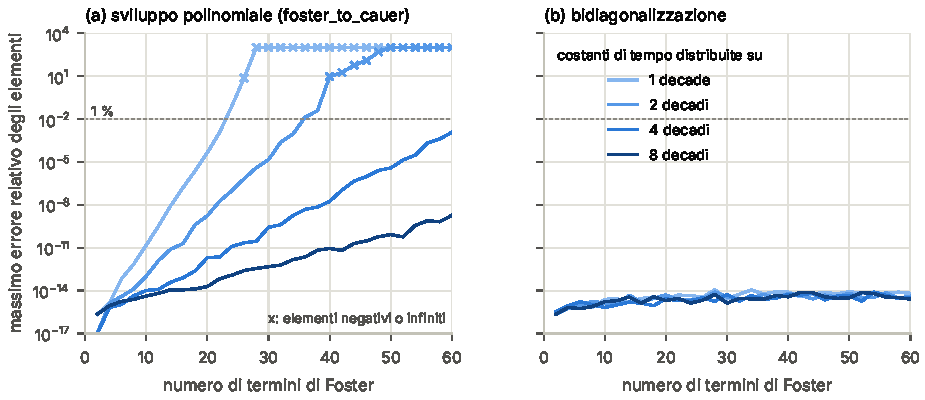
\includegraphics[width=\textwidth]{figures/fig_accuracy_it.pdf}
\caption{Massimo errore relativo degli elementi della rete a scala rispetto al riferimento a \fcmpDigits{} cifre, per $n$ termini di Foster di uguale resistenza con costanti di tempo equispaziate in scala logaritmica su una fino a otto decadi. (a) Sviluppo polinomiale, la funzione \code{foster\_to\_cauer()}: l'errore cresce con la densità delle costanti di tempo; le croci indicano elementi negativi o infiniti (errori oltre $10^3$ tracciati a $10^3$). (b) Bidiagonalizzazione, \eqref{eq:bidiag}: livello dell'arrotondamento ovunque.}
\label{fig:accuracy}
\end{figure}

%=====================================================================
\section{Raffreddamento su due lati: una rete a scala per lato}
\label{sec:sides}

\subsection{La suddivisione}
Un press-pack è raffreddato attraverso entrambi i poli, e i suoi due case possono vedere reti esterne diverse: contatti diversi, una barra da un lato e un dissipatore dall'altro, un dispositivo adiacente. Il datasheet dà una sola impedenza per i due lati insieme, $Z(s)$, e le resistenze a regime per il solo lato anodo e il solo lato catodo, $R_\mathrm{a}$ e $R_\mathrm{c}$. La suddivisione usata nel modello termico prende la rete a scala di $Z$ e ne fa una copia per lato, scalata:
\begin{equation}
\Rpar = \left(\frac{1}{R_\mathrm{a}} + \frac{1}{R_\mathrm{c}}\right)^{-1} , \qquad k_\mathrm{a} = \frac{R_\mathrm{a}}{\Rpar} , \quad k_\mathrm{c} = \frac{R_\mathrm{c}}{\Rpar} ; \qquad
\text{lato } x\!: \ R_k\, k_x \ (k = 1\ldots n) , \quad \frac{C_k}{k_x} \ (k = 2\ldots n) ,
\label{eq:split}
\end{equation}
con il nodo di giunzione e la sua capacità $C_1$ in comune tra i due lati (Fig.~\ref{fig:split}).

Moltiplicare ogni resistenza per $k$ e dividere ogni capacità per $k$ moltiplica per $k$ ogni impedenza della rete a scala, a ogni frequenza. Sia $Z'(s)$ l'impedenza della rete a scala di $Z$ vista dalla giunzione senza $C_1$; le due copie scalate in parallelo hanno l'impedenza
\begin{equation}
\left(\frac{1}{k_\mathrm{a}Z'} + \frac{1}{k_\mathrm{c}Z'}\right)^{-1} = \frac{Z'}{1/k_\mathrm{a} + 1/k_\mathrm{c}} = Z' ,
\qquad\text{poiché}\qquad \frac{1}{k_\mathrm{a}} + \frac{1}{k_\mathrm{c}} = \Rpar\left(\frac{1}{R_\mathrm{a}} + \frac{1}{R_\mathrm{c}}\right) = 1 .
\end{equation}
Con $C_1$ in parallelo, questa è $Z(s)$: con i due case alla stessa temperatura la rete suddivisa ha esattamente l'impedenza con raffreddamento su due lati del datasheet, e la somma delle capacità delle due copie è la capacità della rete a scala. A regime la quota di calore che esce dall'anodo è $1/k_\mathrm{a} = R_\mathrm{c}/(R_\mathrm{a}+R_\mathrm{c})$.

Nella suddivisione entra solo il rapporto $R_\mathrm{a}/R_\mathrm{c}$. Se la $\sum R_i$ della tabella e la $\Rpar$ dei valori su singolo lato differiscono di poco, come di solito accade in un datasheet, le resistenze su singolo lato delle reti a scala suddivise sono $k_x\sum R_i$, non esattamente $R_x$; l'impedenza con raffreddamento su due lati è conservata.

\begin{figure}[htb]
\centering
\begin{circuitikz}[scale=0.8, transform shape, european resistors]
% giunzione, capacità in comune, potenza
\draw (0,-1.4) node[ground]{} to[I, l=$p(t)$, invert] (0,0);
\draw (0,0) node[circ]{} node[above left]{$\Tj$} -- (1.4,0) node[circ]{};
\draw (1.4,0) to[C, l_=$C_1$] (1.4,-1.4) node[ground]{};
\draw (1.4,0) -- (1.4,3.0) -- (2.2,3.0);
\draw (1.4,0) -- (2.2,0);
% lato anodo, riga superiore
\draw (2.2,3.0) to[R, l=$R_1k_\mathrm{a}$] (4.2,3.0) node[circ]{};
\draw (4.2,3.0) to[C, l_=$C_2/k_\mathrm{a}$] (4.2,1.6) node[ground]{};
\draw (4.2,3.0) to[R, l=$R_2k_\mathrm{a}$] (6.4,3.0) node[circ]{};
\draw (6.4,3.0) to[C, l_=$C_3/k_\mathrm{a}$] (6.4,1.6) node[ground]{};
\draw (6.4,3.0) to[R, l=$R_3k_\mathrm{a}$] (8.6,3.0) node[circ]{};
\draw (8.6,3.0) to[C, l_=$C_4/k_\mathrm{a}$] (8.6,1.6) node[ground]{};
\draw (8.6,3.0) to[R, l=$R_4k_\mathrm{a}$] (10.8,3.0) node[circ]{} node[below=3pt]{case a};
\draw (10.8,3.0) to[R, l=$\Rch$] (13.0,3.0) node[circ]{};
\draw (13.0,3.0) to[C, l=barra o dissipatore] (13.0,1.6) node[ground]{};
% lato catodo, riga inferiore
\draw (2.2,0) to[R, l=$R_1k_\mathrm{c}$] (4.2,0) node[circ]{};
\draw (4.2,0) to[C, l_=$C_2/k_\mathrm{c}$] (4.2,-1.4) node[ground]{};
\draw (4.2,0) to[R, l=$R_2k_\mathrm{c}$] (6.4,0) node[circ]{};
\draw (6.4,0) to[C, l_=$C_3/k_\mathrm{c}$] (6.4,-1.4) node[ground]{};
\draw (6.4,0) to[R, l=$R_3k_\mathrm{c}$] (8.6,0) node[circ]{};
\draw (8.6,0) to[C, l_=$C_4/k_\mathrm{c}$] (8.6,-1.4) node[ground]{};
\draw (8.6,0) to[R, l=$R_4k_\mathrm{c}$] (10.8,0) node[circ]{} node[below=3pt]{case c};
\draw (10.8,0) to[R, l=$\Rch$] (13.0,0) node[circ]{};
\draw (13.0,0) to[C, l=barra o dissipatore] (13.0,-1.4) node[ground]{};
\end{circuitikz}
\caption{La rete a scala dell'impedenza con raffreddamento su due lati suddivisa in una rete a scala per lato, \eqref{eq:split}: il nodo di giunzione e $C_1$ sono in comune; ogni lato, anodo in alto e catodo in basso, è il resto della rete a scala con $R\times k$ e $C/k$ e termina al proprio nodo di case, collegato alla propria rete esterna (qui una resistenza di contatto e una barra o un dissipatore a parametri concentrati).}
\label{fig:split}
\end{figure}

\subsection{Che cosa presuppone la suddivisione}
La suddivisione è esatta per l'impedenza con raffreddamento su due lati e per le resistenze su singolo lato, ed è un'ipotesi per tutto il resto. Presuppone che i due percorsi termici abbiano la stessa forma e differiscano solo per un fattore di scala: la stessa distribuzione di resistenza e capacità lungo il percorso, con più dell'una e dell'altra su un lato. In un press-pack reale i lati differiscono negli strati (un disco di molibdeno legato al silicio da un lato, uno flottante dall'altro, poli di spessore diverso) e i loro transitori su singolo lato non sono proporzionali. Il datasheet non dà abbastanza per fare di meglio: le curve su singolo lato, quando il datasheet le riporta, sono misurate con l'altro lato adiabatico e contengono il calore accumulato nel lato che non raffredda, per cui non si può fare il fit di ciascun lato da solo. Un'identificazione coerente farebbe il fit delle due reti a scala insieme sulle tre curve; la suddivisione scalata è ciò che resta quando sono dati solo la tabella con raffreddamento su due lati e due resistenze. La Sez.~\ref{sec:synthetic} ne misura il costo.

Quando il datasheet non dà valori su singolo lato, la scelta naturale è $k_\mathrm{a} = k_\mathrm{c} = 2$, lati uguali, dichiarata come ipotesi.

\subsection{Le reti a scala in un modello termico}
La verifica termica per cui la funzione è stata scritta usa la suddivisione così: il nodo di giunzione con $C_1$; per ogni lato i tre nodi interni con $C_k/k$ e le quattro resistenze $R_kk$; un nodo di case senza capacità; la resistenza di contatto di ciascun lato distribuita sulle celle della barra sotto il polo; la barra come modello tridimensionale ai volumi finiti del rame, adiabatico sulle facce libere. Le perdite $p = V_\mathrm{T0}|i| + r_\mathrm{T}i^2$ sono iniettate nel nodo di giunzione e l'intero sistema lineare $\mathbf{C}\dot{\mathbf{T}} = -G\mathbf{T} + \mathbf{b}\,p(t)$ è integrato con un metodo implicito. Una simulazione con i nodi di case collegati a un dissipatore ideale deve restituire $\Zjc$: è la prima verifica di un modello di questo tipo.

%=====================================================================
\section{Esempi svolti: due dispositivi press-pack}
\label{sec:examples}

\subsection{Dati}
I due dispositivi sono un diodo raddrizzatore di classe \SI{2}{\kilo\volt}, \fcddRth~\KkW{} giunzione--case con raffreddamento su due lati, \SI{14.5}{\kelvin\per\kilo\watt} dal lato anodo e \SI{18.0}{\kelvin\per\kilo\watt} dal lato catodo; e un tiristore a controllo di fase di classe \SI{1.8}{\kilo\volt}, \fcdtRth~\KkW{} con raffreddamento su due lati, per il quale si assumono lati uguali. Le tabelle a quattro termini sono quelle dei rispettivi datasheet (Tab.~\ref{tab:cauer}).

\begin{table}[htb]
\centering\small
\caption{Tabelle di Foster dei datasheet (raffreddamento su due lati) e reti a scala di Cauer ottenute con \code{foster\_to\_cauer()}. $C^\mathrm{F} = \tau/R$ sono le capacità delle celle di Foster, $\theta_k$ la resistenza dal nodo $k$ al case.}
\label{tab:cauer}
\begin{tabular}{@{}l l c c c @{\hspace{1.4em}} c c c c@{}}
\toprule
& & \multicolumn{3}{c}{Foster (datasheet)} & \multicolumn{4}{c}{Cauer} \\
\cmidrule(lr){3-5}\cmidrule(l){6-9}
& $i$, $k$ & {$R_i$ (\KkW)} & {$\tau_i$ (\si{\second})} & {$C^\mathrm{F}_i$ (\JK)} & {$R_k$ (\KkW)} & {$C_k$ (\JK)} & {$R_kC_k$ (\ms)} & {$\theta_k$ (\KkW)} \\
\midrule
5SDD 70H2000 & 1 & \fcddRA & \fcddTA & \fcddCfA & \fcddRcA & \fcddCcA & \fcddRCcA & \fcddThetaA \\
diodo        & 2 & \fcddRB & \fcddTB & \fcddCfB & \fcddRcB & \fcddCcB & \fcddRCcB & \fcddThetaB \\
             & 3 & \fcddRC & \fcddTC & \fcddCfC & \fcddRcC & \fcddCcC & \fcddRCcC & \fcddThetaC \\
             & 4 & \fcddRD & \fcddTD & \fcddCfD & \fcddRcD & \fcddCcD & \fcddRCcD & \fcddThetaD \\
             & somma & \fcddRth & & \fcddCfSum & \fcddRth & \fcddCcSum & & \\
\midrule
5STP 50Q1800 & 1 & \fcdtRA & \fcdtTA & \fcdtCfA & \fcdtRcA & \fcdtCcA & \fcdtRCcA & \fcdtThetaA \\
tiristore    & 2 & \fcdtRB & \fcdtTB & \fcdtCfB & \fcdtRcB & \fcdtCcB & \fcdtRCcB & \fcdtThetaB \\
             & 3 & \fcdtRC & \fcdtTC & \fcdtCfC & \fcdtRcC & \fcdtCcC & \fcdtRCcC & \fcdtThetaC \\
             & 4 & \fcdtRD & \fcdtTD & \fcdtCfD & \fcdtRcD & \fcdtCcD & \fcdtRCcD & \fcdtThetaD \\
             & somma & \fcdtRth & & \fcdtCfSum & \fcdtRth & \fcdtCcSum & & \\
\bottomrule
\end{tabular}
\end{table}

\subsection{Le reti a scala}
La Tab.~\ref{tab:cauer} e la Fig.~\ref{fig:datasheet} riportano il risultato. Alcuni punti valgono al di là di questi due dispositivi:
\begin{itemize}
\item Le reti a scala si leggono dalla giunzione verso l'esterno: una piccola capacità alla giunzione (\fcddCcA{} e \fcdtCcA~\JK, il silicio e ciò che gli sta vicino), poi capacità più grandi, e la più grande all'ultimo nodo, vicino al case (\fcddCcD{} e \fcdtCcD~\JK, i poli). Le capacità di Foster vanno nel verso opposto, la più grande nella cella più lenta; non dicono nulla su dove si accumuli il calore.
\item I prodotti $R_kC_k$ non sono le costanti di tempo di Foster. Le costanti di tempo della rete a scala sono date dai suoi autovalori \eqref{eq:eig}, e sono le $\tau_i$.
\item Le verifiche della Sez.~\ref{sec:checks} sono soddisfatte a meno dell'arrotondamento: $C_1$ è uguale a $1/\sum (R_i/\tau_i) = 1/\sum(1/C^\mathrm{F}_i) = \fcddCfSeries$~\JK{} per il diodo e a \fcdtCfSeries~\JK{} per il tiristore; $R_1$ è uguale alla \eqref{eq:first}; $\sum_i R_i\tau_i = \sum_k C_k\theta_k^2 = \fcddMone$ e \fcdtMone~\si{\kelvin\second\per\kilo\watt}. Lo sviluppo polinomiale concorda con il riferimento a \fcmpDigits{} cifre entro $\fcddErrPoly$ (diodo) e $\fcdtErrPoly$ (tiristore), la bidiagonalizzazione entro $\fcddErrBid$ e $\fcdtErrBid$, l'andata e ritorno \eqref{eq:eig} restituisce la tabella entro $\fcddErrRt$ e $\fcdtErrRt$, e le risposte al gradino di rete a scala e tabella concordano entro $\fcddErrZ$ da \SI{1}{\micro\second} a \SI{1000}{\second} (Fig.~\ref{fig:datasheet}a).
\item A regime il diodo accumula \fcddStored~J, il tiristore \fcdtStored~J, per kilowatt di perdite ($\sum_k C_k\theta_k$): in media il calore lascia il case \fcddDelay~s e \fcdtDelay~s dopo essere stato generato. La rete di Foster non ha alcun ritardo di questo tipo.
\end{itemize}
Tracciata come capacità cumulata in funzione della resistenza cumulata dalla giunzione (Fig.~\ref{fig:datasheet}b), una rete a scala è una scalinata: la funzione di struttura cumulativa nella sua forma più grossolana \cite{szekely1988,szekely1997}. I tratti piatti sono resistenza senza capacità termica (contatti, strati sottili), i tratti ripidi capacità termica dietro poca resistenza (i poli).

\begin{figure}[htb]
\centering
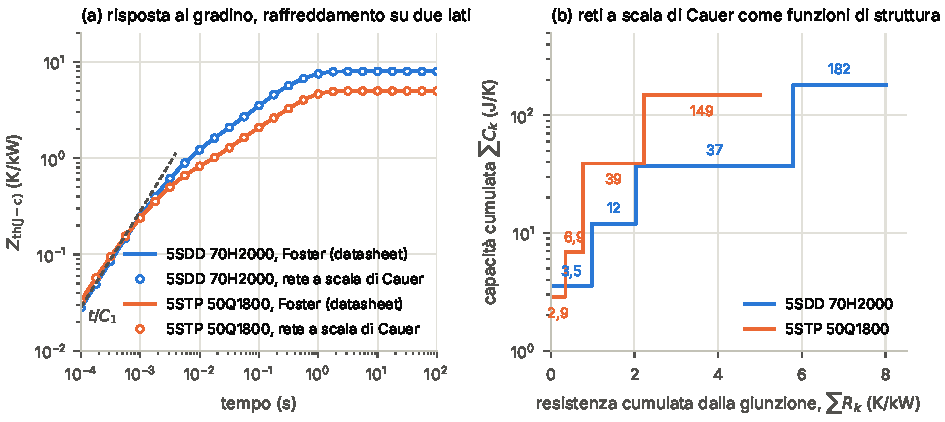
\includegraphics[width=\textwidth]{figures/fig_datasheet_it.pdf}
\caption{I due dispositivi della Tab.~\ref{tab:cauer}. (a) Risposta al gradino della tabella del datasheet (linee) e della rete a scala di Cauer (cerchi), con raffreddamento su due lati; la linea tratteggiata è $t/C_1$ del diodo, l'inizio di ogni rete con questa impedenza. (b) Le reti a scala come funzioni di struttura: capacità cumulata in funzione della resistenza cumulata dalla giunzione, con la capacità cumulata di ogni gradino.}
\label{fig:datasheet}
\end{figure}

\subsection{Una rete a scala per lato}
Per il diodo $\Rpar = \fcddRpar$~\KkW, $k_\mathrm{a} = \fcddKa$ e $k_\mathrm{c} = \fcddKb$, e a regime il \fcddShareA~\% del calore esce dall'anodo. Le due reti a scala \eqref{eq:split} sono nella Tab.~\ref{tab:sides}; le loro resistenze su singolo lato sono \fcddRsSuma{} e \fcddRsSumb~\KkW{} invece di \num{14.5} e \num{18.0}, perché la tabella ha somma \fcddRth~\KkW{} e il parallelo dei valori su singolo lato è \fcddRpar~\KkW. Per il tiristore, con lati uguali per ipotesi, $k = 2$: ogni lato è la rete a scala con resistenze raddoppiate e capacità dimezzate.

\begin{table}[htb]
\centering\small
\caption{Reti a scala per lato del diodo, \eqref{eq:split}. La capacità di giunzione $C_1 = \fcddCcA$~\JK{} è in comune.}
\label{tab:sides}
\begin{tabular}{@{}l c c c c @{\hspace{1.5em}} c c c@{}}
\toprule
lato & {$R_1k$} & {$R_2k$} & {$R_3k$} & {$R_4k$ (\KkW)} & {$C_2/k$} & {$C_3/k$} & {$C_4/k$ (\JK)} \\
\midrule
anodo, $k_\mathrm{a} = \fcddKa$ & \fcddRsaA & \fcddRsaB & \fcddRsaC & \fcddRsaD & \fcddCsaB & \fcddCsaC & \fcddCsaD \\
catodo, $k_\mathrm{c} = \fcddKb$ & \fcddRsbA & \fcddRsbB & \fcddRsbC & \fcddRsbD & \fcddCsbB & \fcddCsbC & \fcddCsbD \\
\bottomrule
\end{tabular}
\end{table}

\subsection{Il diodo tra due barre di rame}
\label{sec:onbars}
Per vedere che cosa cambia con la rete a scala, il diodo è serrato tra due barre di rame da \fccpCbar~\JK{} ciascuna (una barra $100 \times 10 \times \SI{180}{\milli\metre}$), a parametri concentrati e adiabatiche, attraverso un contatto di \fccpRch~\KkW{} per lato, e dissipa \SI{\fccpP}{\kilo\watt} per \SI{\fccpT}{\second} (\SI{\fccpE}{\kilo\joule}). Si confrontano tre modelli del dispositivo (Fig.~\ref{fig:coupling}):
\begin{itemize}
\item la rete a scala di Cauer suddivisa per lato, ciascun case sul proprio contatto e sulla propria barra;
\item la tabella di Foster con un solo nodo di case, collegato a entrambi i contatti e a entrambe le barre;
\item la tabella di Foster su un dissipatore ideale, come riferimento.
\end{itemize}
Alla fine dell'impulso la giunzione si è innalzata di \SI{\fccpTjC}{\kelvin} con le reti a scala, di \SI{\fccpTjF}{\kelvin} con la tabella di Foster sulle barre e di \SI{\fccpTjI}{\kelvin} sul dissipatore ideale. La differenza sta nel case. Con la tabella di Foster l'intera potenza attraversa i contatti fin dal primo istante: il case salta subito a \SI{\fccpTcFzero}{\kelvin} e termina a \SI{\fccpTcF}{\kelvin}. Con la rete a scala il calore verso le barre parte da zero, raggiunge il \SI{10}{\percent} della potenza dopo \SI{\fccpQten}{\milli\second} e il \SI{\fccpQend}{\percent} alla fine dell'impulso; \SI{\fccpEstored}{\kilo\joule} dei \SI{\fccpE}{\kilo\joule} (\SI{\fccpEstoredPct}{\percent}) sono ancora nel dispositivo, e il case più caldo si è innalzato di \SI{\fccpTcC}{\kelvin}. Dopo l'impulso il calore accumulato fluisce nelle barre e la giunzione si raffredda più lentamente che con la tabella di Foster, che a quel punto ha già messo tutta l'energia nelle barre.

Qui la tabella di Foster sulle barre non sbaglia nella direzione pericolosa: è troppo pessimistica, di \SI{\fccpDiff}{\kelvin} su un margine calcolato rispetto a un limite di giunzione; il dissipatore ideale, all'estremo opposto, ignora il riscaldamento del case. La rete a scala sta tra i due, vicina al dissipatore ideale per questo impulso perché in mezzo secondo poco calore raggiunge le barre.

\begin{figure}[htb]
\centering
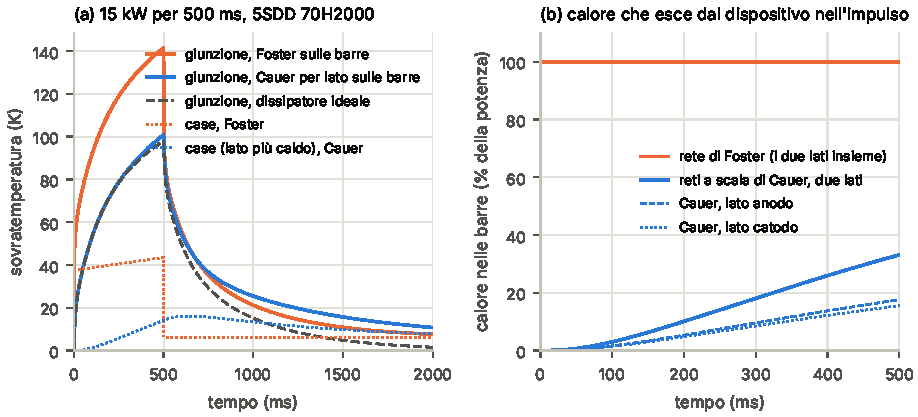
\includegraphics[width=\textwidth]{figures/fig_coupling_it.pdf}
\caption{Diodo della Tab.~\ref{tab:cauer} tra due barre di rame (\fccpCbar~\JK{} e contatto di \fccpRch~\KkW{} per lato), \SI{\fccpP}{\kilo\watt} per \SI{\fccpT}{\second}. (a) Sovratemperatura di giunzione e di case con le reti a scala di Cauer per lato, con la tabella di Foster collegata alle barre attraverso un solo nodo di case, e con un dissipatore ideale. (b) Calore che fluisce nelle barre durante l'impulso, come quota della potenza.}
\label{fig:coupling}
\end{figure}

%=====================================================================
\section{Verifica su un press-pack con strati noti}
\label{sec:synthetic}
Gli esempi della Sez.~\ref{sec:examples} mostrano la differenza tra le reti ma non quale sia quella giusta, perché il dispositivo reale non è noto. Un press-pack sintetico lo è: un modello monodimensionale alle differenze finite degli strati, la cui impedenza transitoria esatta fa le veci della misura del datasheet e la cui risposta sulle barre fa le veci della realtà.

\subsection{Il modello}
Il dispositivo ha l'area di un polo da \SI{63}{\milli\metre} e, dal case anodo al case catodo: polo di rame da \SI{8}{\milli\metre}; contatto da \SI{2.5}{\kelvin\per\kilo\watt}; molibdeno da \SI{2}{\milli\metre} legato al silicio; silicio da \SI{0.5}{\milli\metre}; contatto da \SI{4}{\kelvin\per\kilo\watt}; molibdeno da \SI{1.5}{\milli\metre}; contatto da \SI{2.5}{\kelvin\per\kilo\watt}; polo di rame da \SI{8}{\milli\metre}. Conducibilità termiche \num{390}, \num{138} e \SI{120}{\watt\per\metre\per\kelvin}, capacità termiche volumiche dalle densità e dai calori specifici di rame, molibdeno e silicio. Le perdite sono distribuite uniformemente nel silicio e la temperatura di giunzione è la temperatura media del silicio, come lo sarebbe una temperatura virtuale di giunzione. Il modello ha \fcsyNodes{} celle; capacità termiche: silicio \fcsyCsi; molibdeno \fcsyCmo; rame \fcsyCcu~\JK; in totale \fcsyCtot~\JK. Con entrambe le facce a temperatura costante $\Rjc = \fcsyRth$~\KkW; con il solo lato anodo \fcsyRa{} e con il solo lato catodo \fcsyRc~\KkW. Una seconda variante ha i lati uguali (il lato catodo realizzato come il lato anodo), per separare ciò che deriva dalla suddivisione.

L'impedenza esatta del modello è una somma di Foster dei suoi modi (\fcsyModes{} termini con peso superiore a $10^{-12}$ del totale, costanti di tempo da \SI{9}{\micro\second} a \SI{0.34}{\second}). La sua rete a scala esatta, ottenuta con la bidiagonalizzazione (qui lo sviluppo polinomiale restituisce elementi negativi), restituisce l'impedenza entro $\fcsyErrFull$. Come farebbe un datasheet, l'impedenza è poi campionata da \SI{1}{\milli\second} a \SI{10}{\second} e approssimata con fit di Foster da tre a sei termini; il fit a quattro termini si scosta dalla curva entro \SI{\fcsyFitFourErr}{\percent} nella finestra.

\subsection{Funzione di struttura}
La Fig.~\ref{fig:synthetic}b mostra la rete a scala esatta come funzione di struttura insieme alla capacità termica cumulata degli strati. La rete li segue: un gradino di circa \fcsyCsi~\JK{} per il silicio, il molibdeno, un tratto piatto attraverso i contatti, la salita ripida del rame; fino al \SI{99}{\percent} di $\Rjc$ la capacità cumulata è \fcsyCninetyNine~\JK{} contro i \fcsyCtot~\JK{} degli strati. Poi la curva diventa verticale: l'ultima resistenza è mantenuta a temperatura costante dall'altro lato, il che nella funzione di struttura equivale a una capacità infinita.

Le reti a scala dei fit sono scalinate grossolane della stessa curva. La loro capacità totale è \fcsyFitThreeCsum, \fcsyFitFourCsum, \fcsyFitFiveCsum{} e \fcsyFitSixCsum~\JK{} per tre, quattro, cinque e sei termini, da un terzo a due terzi della capacità termica degli strati. Manca il rame vicino alle facce. Con le facce a temperatura costante quel rame resta quasi alla loro temperatura, accumula poco calore e quasi non cambia la curva, per cui un fit sulla finestra misurata non lo vede; più termini ci sono, più la rete a scala ne recupera. La capacità di giunzione è il numero più robusto: \fcsyFitFourCo~\JK{} dal fit a quattro termini contro \fcsyCsi~\JK{} del silicio.

\begin{figure}[htb]
\centering
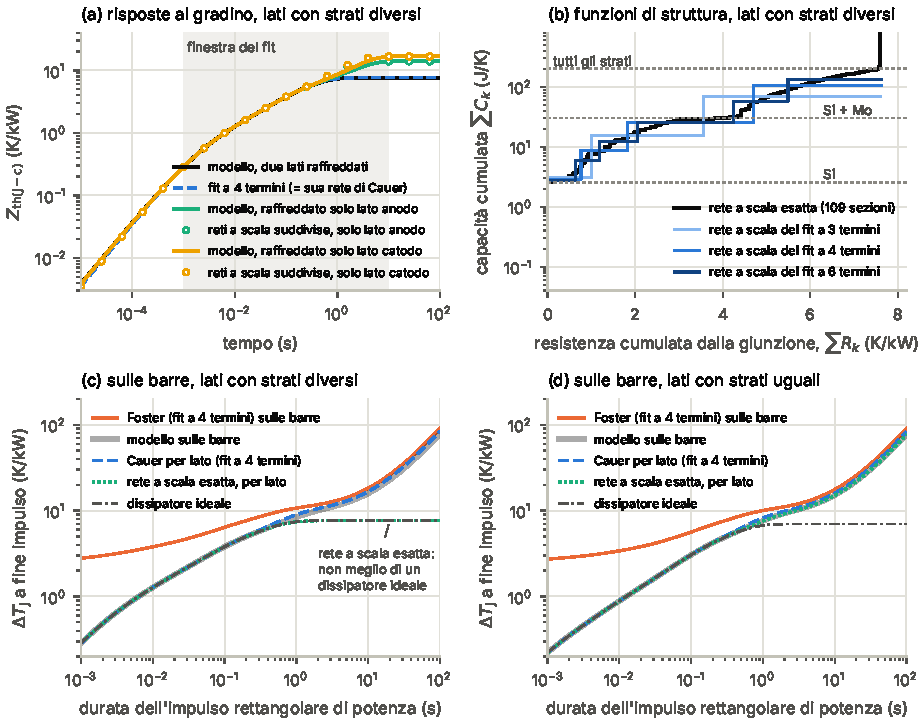
\includegraphics[width=\textwidth]{figures/fig_synthetic_it.pdf}
\caption{Press-pack sintetico. (a) Risposte al gradino del modello con entrambi i lati raffreddati e con un solo lato, il fit a quattro termini sulla finestra, e le curve su singolo lato delle reti a scala suddivise di quel fit. (b) Rete a scala esatta del modello e reti a scala dei fit come funzioni di struttura; linee punteggiate: capacità termica cumulata degli strati. (c), (d) Sovratemperatura di giunzione per kilowatt alla fine di un impulso rettangolare con il dispositivo tra due barre (\fccpCbar~\JK, \fccpRch~\KkW{} per lato): modello, reti a scala di Cauer per lato, tabella di Foster sulle barre, dissipatore ideale; (c) lati con strati diversi, (d) lati uguali.}
\label{fig:synthetic}
\end{figure}

\subsection{Sulle barre}
Il dispositivo è posto tra le due barre della Sez.~\ref{sec:onbars} e la sovratemperatura di giunzione alla fine di un impulso rettangolare è confrontata con il modello (Fig.~\ref{fig:synthetic}c e~d, Tab.~\ref{tab:synthetic}).

\begin{table}[htb]
\centering\small
\caption{Press-pack sintetico tra due barre: sovratemperatura di giunzione per kilowatt alla fine di un impulso di \SI{0.5}{\second}, suo scostamento dal modello, e massimo scostamento per impulsi da \SI{1}{\milli\second} a \SI{100}{\second}.}
\label{tab:synthetic}
\begin{tabular}{@{}l c c c @{\hspace{1.5em}} c c c@{}}
\toprule
& \multicolumn{3}{c}{lati con strati diversi} & \multicolumn{3}{c}{lati uguali} \\
\cmidrule(lr){2-4}\cmidrule(l){5-7}
& {\SI{0.5}{\second}, \KkW} & {scost., \%} & {max., \%} & {\SI{0.5}{\second}, \KkW} & {scost., \%} & {max., \%} \\
\midrule
modello (realtà) & \fcsyHalfZm & & & \fcssHalfZm & & \\
Cauer per lato, fit a 4 termini & \fcsyHalfZc & \fcsyHalfEc & \fcsyMaxEc & \fcssHalfZc & \fcssHalfEc & \fcssMaxEc \\
Cauer per lato, rete a scala esatta & \fcsyHalfZx & \fcsyHalfEx & \fcsyMaxEx & \fcssHalfZx & \fcssHalfEx & \fcssMaxEx \\
Foster sulle barre, fit a 4 termini & \fcsyHalfZf & \fcsyHalfEf & \fcsyMaxEf & \fcssHalfZf & \fcssHalfEf & \fcssMaxEf \\
dissipatore ideale & \fcsyHalfZi & \fcsyHalfEi & & \fcssHalfZi & \fcssHalfEi & \\
\bottomrule
\end{tabular}
\end{table}

\begin{itemize}
\item La rete a scala del fit a quattro termini, suddivisa per lato, segue il modello entro \SI{0.3}{\percent} per impulsi fino a \SI{0.1}{\second}, ed è più alta del \SIrange{5}{7}{\percent} per impulsi più lunghi, in entrambe le varianti: al massimo \fcsyMaxEc~\% con i lati diversi, \fcssMaxEc~\% con i lati uguali. Con tre, cinque e sei termini il massimo scostamento è rispettivamente \fcsyFitThreeDev{}; \fcsyFitFiveDev{} e \fcsyFitSixDev~\%: si riduce man mano che la rete a scala recupera la capacità vicino alle facce.
\item La tabella di Foster sulle barre è più alta del \SI{\fcsyHalfEf}{\percent} a \SI{0.5}{\second} e molto di più per impulsi brevi, quando la sovratemperatura di giunzione è piccola mentre la caduta sul contatto dovuta all'intera potenza non lo è: a \SI{10}{\milli\second} vale da tre a quattro volte il modello.
\item Il dissipatore ideale è corretto fino a circa \SI{0.1}{\second} e poi sempre più basso.
\end{itemize}

\subsection{Che cosa la rete a scala non contiene}
\label{sec:missing}
Tre effetti spiegano gli scostamenti, e conviene tenerli presenti per ogni rete a scala ricavata da un datasheet.

\emph{Capacità termica vicino al case.} La prova con il case a temperatura costante è insensibile alla capacità termica vicina al case, per cui la rete a scala ottenuta dal fit ne ha meno del dispositivo. Su un dissipatore che si scalda quella capacità assorbirebbe calore; senza di essa la giunzione risulta qualche punto percentuale troppo calda. L'errore è a favore di sicurezza.

\emph{Transitori su singolo lato.} La stessa capacità mancante pesa di più quando una faccia è adiabatica: il lato che non raffredda si scalda nel suo insieme, tutto il suo rame assorbe calore, e nella rete a scala quel rame non c'è. Le reti a scala suddivise del fit a quattro termini danno curve su singolo lato fino al \SI{\fcsySaDevF}{\percent} troppo alte intorno a \SI{\fcsySaDevT}{\second}, anche con lati uguali (\SI{\fcssSaDevF}{\percent}); il loro regime è corretto a meno della piccola differenza tra $\sum R_i$ e $\Rpar$. Con la rete a scala esatta del dispositivo a lati uguali le curve su singolo lato sono entro \SI{\fcssSaAbsX}{\percent} dal modello: la suddivisione in sé è esatta quando i lati sono proporzionali, e l'errore viene dal fit.

\emph{La rete a scala esatta di lati diversi.} Quando i lati differiscono, la rete a scala esatta dell'impedenza con raffreddamento su due lati è un unico percorso che ne imita due diversi. Segue gli strati fin quasi a tutta la $\Rjc$ (Fig.~\ref{fig:synthetic}b) e poi termina con sezioni di resistenza piccolissima e capacità fino a $\fcsyCmax$~\JK, che non corrispondono ad alcun materiale. Con il case a temperatura costante sono innocue. Sulle barre agiscono come un secondo dissipatore: la giunzione segue la curva del dissipatore ideale ed è fino al \SI{\fcsyMaxEx}{\percent} troppo fredda per impulsi lunghi (Fig.~\ref{fig:synthetic}c), e le sue curve su singolo lato restano molto al di sotto delle resistenze su singolo lato (\SI{\fcsySaDevX}{\percent} a \SI{50}{\second}). Con lati uguali la rete a scala esatta non ha sezioni di questo tipo e segue il modello entro \SI{\fcssMaxEx}{\percent} (Fig.~\ref{fig:synthetic}d). Una rete a scala ricavata da un fit di pochi termini, come da un datasheet, non sviluppa il problema; una rete a scala ricavata da un'analisi fine con le funzioni di struttura di una misura con raffreddamento su due lati va troncata dove la funzione di struttura diventa verticale, prima di collegarla a qualsiasi cosa.

Al di sotto della finestra del fit vale il contrario: la rete estrapola la curva con la pendenza $t/C_1$, mentre un dispositivo reale segue $\sqrt{t}$ \cite{activeclamping}. A \SI{100}{\micro\second} il fit a quattro termini si scosta dal modello di \SI{\fcsyShortA}{\percent}, a \SI{10}{\micro\second} di \SI{\fcsyShortB}{\percent}: troppo basso, a sfavore di sicurezza, per impulsi più brevi della costante di tempo più rapida della tabella.

%=====================================================================
\section{Procedura}
\label{sec:procedure}
\begin{enumerate}
\item Prendere dal datasheet la tabella di Foster di $\Zjc$, con raffreddamento su due lati per un press-pack, e verificare che $\sum R_i$ sia uguale alla $\Rjc$ del datasheet. Annotare la finestra temporale della curva: al di sotto la tabella è un'estrapolazione.
\item Convertirla con \code{foster\_to\_cauer()} (fino a una dozzina di termini) o con \code{foster\_to\_cauer\_bidiag()} (qualsiasi numero). Verificare che tutti gli elementi siano positivi, che $\sum R_k = \sum R_i$, $C_1 = 1/\sum (R_i/\tau_i)$, $\sum C_k\theta_k^2 = \sum R_i\tau_i$, e che l'andata e ritorno \eqref{eq:eig} restituisca la tabella.
\item Per un dispositivo raffreddato su due lati i cui lati vedono reti esterne diverse, suddividere la rete a scala con le resistenze su singolo lato del datasheet, \eqref{eq:split}. In mancanza di valori su singolo lato, assumere lati uguali e dichiararlo.
\item Collegare ogni nodo di case alla propria rete esterna: resistenza di contatto per lato, poi il dissipatore o il modello della barra. Non collegare una rete di Foster a nient'altro che a una temperatura costante.
\item Eseguire il modello una volta con i nodi di case a temperatura costante: deve riprodurre $\Zjc$.
\item Calcolare le perdite dalla corrente con i parametri di conduzione alla massima temperatura di giunzione, iniettarle nel nodo di giunzione, integrare.
\item Leggere la temperatura di giunzione tenendo presenti i limiti della rete a scala: qualche punto percentuale in eccesso su un dissipatore che si scalda, di più nei transitori con raffreddamento su un solo lato, troppo bassa per impulsi più brevi della costante di tempo più rapida della tabella.
\end{enumerate}

%=====================================================================
\appendix
\section{Script di supporto}
\label{sec:scripts}
\begin{itemize}
\item \code{foster\_cauer.py} è un modulo con le relazioni della nota, in unità SI (K/W, s, J/K): le conversioni \code{foster\_to\_cauer} (la funzione della Sez.~\ref{sec:code}, invariata nei suoi passi), \code{foster\_to\_cauer\_mp} (gli stessi passi con \fcmpDigits{} cifre, come riferimento), \code{foster\_to\_cauer\_bidiag} (Sez.~\ref{sec:bidiag}) e \code{cauer\_to\_foster} (Sez.~\ref{sec:inverse}); le risposte al gradino \code{zth\_foster} e \code{zth\_cauer}; le verifiche \code{invariants} e \code{ladder\_moment}; la suddivisione \code{split\_sides}; la scalinata \code{structure\_function}; e una classe \code{Network} che assembla nodi, reti a scala, contatti e dissipatori e ne calcola la risposta esatta a una potenza costante a tratti a partire dagli autovalori della rete (i nodi senza capacità vengono eliminati prima). Eseguito come programma, confronta tra loro le tre conversioni.
\item \code{foster\_cauer\_calc.py} contiene in testa i dati degli esempi e produce i numeri e le figure della nota: il log \code{foster\_cauer\_results.txt}, il file \code{foster\_cauer\_values.tex} con ogni numero qui citato in forma di macro (lo stesso per la versione inglese e per questa, che lo legge con la virgola decimale), e le figure \code{figures/*.pdf} con le etichette in inglese e \code{figures/*\_it.pdf} con le etichette in italiano. Gira in una ventina di secondi. Per convertire un altro dispositivo, sostituire una tabella in \code{DIODE} o \code{THYR}; la rete esterna degli esempi è fissata da \code{R\_CH} e \code{C\_BAR}, il dispositivo sintetico da \code{LAYERS}.
\end{itemize}

%=====================================================================
\begin{thebibliography}{99}
\small
\item[] I riferimenti contrassegnati con [M] sono citati a memoria: i loro dati bibliografici, e le affermazioni tratte da essi, vanno verificati sulla fonte prima dell'uso in un documento di progetto. Le tabelle dei datasheet sono state prese dai datasheet dei dispositivi così come usate nella verifica termica per cui la funzione è stata scritta.

\bibitem{foster1924}
[M] R.~M.~Foster, ``A reactance theorem'', \emph{Bell System Technical Journal}, vol.~3, no.~2, pp.~259--267, 1924.

\bibitem{cauer1926}
[M] W.~Cauer, ``Die Verwirklichung von Wechselstromwiderst\"anden vorgeschriebener Frequenzabh\"angigkeit'', \emph{Archiv f\"ur Elektrotechnik}, vol.~17, pp.~355--388, 1926. Forme canoniche a scala delle impedenze di ingresso.

\bibitem{guillemin1957}
[M] E.~A.~Guillemin, \emph{Synthesis of Passive Networks}, Wiley, 1957. Proprietà delle funzioni di ingresso RC: alternanza di poli e zeri, forme di Foster e di Cauer.

\bibitem{szekely1988}
[M] V.~Sz\'ekely, T.~Van~Bien, ``Fine structure of heat flow path in semiconductor devices: a measurement and identification method'', \emph{Solid-State Electronics}, vol.~31, no.~9, pp.~1363--1368, 1988.

\bibitem{szekely1997}
[M] V.~Sz\'ekely, ``A new evaluation method of thermal transient measurement results'', \emph{Microelectronics Journal}, vol.~28, no.~3, pp.~277--292, 1997. Spettro delle costanti di tempo, trasformazione Foster--Cauer e funzioni di struttura.

\bibitem{jesd5114}
[M] JEDEC, \emph{JESD51-14: Transient Dual Interface Test Method for the Measurement of the Thermal Resistance Junction to Case of Semiconductor Devices with Heat Flow Through a Single Path}, 2010.

\bibitem{golubkahan1965}
[M] G.~H.~Golub, W.~Kahan, ``Calculating the singular values and pseudo-inverse of a matrix'', \emph{SIAM Journal on Numerical Analysis, Series B}, vol.~2, no.~2, pp.~205--224, 1965.

\bibitem{paige1982}
[M] C.~C.~Paige, M.~A.~Saunders, ``LSQR: an algorithm for sparse linear equations and sparse least squares'', \emph{ACM Transactions on Mathematical Software}, vol.~8, no.~1, pp.~43--71, 1982. La bidiagonalizzazione inferiore (\emph{Bidiag 1}) usata nella Sez.~\ref{sec:bidiag}.

\bibitem{gragg1984}
[M] W.~B.~Gragg, W.~J.~Harrod, ``The numerically stable reconstruction of Jacobi matrices from spectral data'', \emph{Numerische Mathematik}, vol.~44, pp.~317--335, 1984.

\bibitem{gautschi2004}
[M] W.~Gautschi, \emph{Orthogonal Polynomials: Computation and Approximation}, Oxford University Press, 2004. Condizionamento del passaggio dai momenti ai coefficienti di ricorrenza.

\bibitem{activeclamping}
pwr-control, \emph{Active clamping of high-voltage IGBTs: theory, design for a 6.5 kV / 1000 A module and a Simscape TVS model}, \texttt{research/power\_electronics/active\_clamping} di questo repository: capacità termica efficace $\bigl(\sum_i R_i/\tau_i\bigr)^{-1}$ di una tabella di Foster e legge in $\sqrt{t}$ ai tempi brevi.

\end{thebibliography}

\end{document}
